\documentclass[a4paper,8pt]{article}
\usepackage[lmargin=20mm,rmargin=20mm,tmargin=20mm,bmargin=20mm]{geometry}
\usepackage{multicol}
\usepackage{graphicx}
\usepackage[labelfont=bf]{caption}
\usepackage{amsmath,amssymb}
\usepackage{physics}
\DeclareMathOperator{\mean}{mean}
\DeclareMathOperator{\van}{van}
\DeclareMathOperator{\aucov}{aucov}


\title{\small FYS9411 -- Computational Physics II \\
\Huge Variational Monte Carlo\\\huge on Elliptical Harmonic Traps with $N$ Bosons}
\author{\large Jonas Boym Flaten \\
\small University of Oslo}
\date{\today}

\begin{document}

\begin{multicols}{2}
[
\maketitle
\begin{abstract}
Using the Julia language, the method of Variational Monte Carlo (VMC) was implemented for a $D$-dimensional elliptical harmonic trap system with $N$ bosons, both with and without interaction. 2 variational parameters were tuned using the gradient descent method to obtain an estimate of the ground state energy for traps with $N = \{10,50,100\}$ bosons. The results are mainly benchmarked against \cite{SWL} which considered the same system but implemented the VMC method in C++ and only varies 1 variational parameter. A comparison of the results from two different Monte Carlo sampling methods, as well as statistical refinement of the results, is presented. Importance sampling using Langevin "quantum drift" sampling is shown to be superior to brute-force "random step" sampling. Finally, the effect of boson interaction is discussed. 
\end{abstract}
]

\section{Introduction}
As far as current human knowledge goes, Quantum Mechanics seems to be an excellent model of the universe at the smallest scales. In this "picoscopic" regime our world can be thought to consist of fuzzy elementary particles, spreading diffusely through space but exchanging sharp energy quanta through four fundamental mechanisms. One big caveat however is the rate at which a thorough quantum mechanical analysis becomes impossible to conduct. For anything more than 1 particle, the complexity of the system of differential equations to consider quickly becomes overwhelming. Add several interaction mechanisms at once and you are sure to end up with a problem that nobody on Earth has been able to solve analytically (yet).

These difficulties with analytical analysis of quantum many-body systems encourages consideration of statistical and numerical methods. With the 
currently available computational power in one's own office and the advent of collaborative development of code over the Internet, the field of Computational Physics has emerged as a third alternative to the traditional theoretical and experimental branches of research. Especially within Quantum Mechanics, where the theoreticists face the complexity of coupled differential systems as discussed above while the experimentalists deal with the frailty (and cost) of experiments tuned to the extreme parameters of the quantum world, computational research is in many cases better suited to the task. Through numerical simulations founded on statistical methods and analysis, large quantum mechanical systems can be explored with remarkable precision.

In this report, the computational method of Variational Monte Carlo (VMC) on an elliptical harmonic trap system containing $N$ bosons is considered, and its implementation in Julia and subsequent results are reported and benchmarked against the previous work of \cite{SWL} and others on the same system. The system is itself interesting because ---noe om bosonisk samfall, noen referanser til forskning på systemet?--- as demonstrated by the famous experiment of \cite{AEMWC}. VMC treatment of this system is discussed by \cite{DBG}, which in turn serves as the inspiration for the work in this report.

Sections \ref{model} and \ref{theory} provide the concrete mathematical model for the system in consideration and the principles leading up to the VMC method. In section \ref{method} the actual Julia implementation as well as the scientific approach to the problem is described. Finally in section \ref{results} the results are presented, discussed and compared to the results of \cite{SWL}.



\section{Model} \label{model}
The model system considered in the project is declared in this chapter.

\subsection{Quantum system}\label{system}
The quantum system considered here is a $D$-dimensional quantum trap with an arbitrary number of identical bosons $N$. In position basis the system Hamiltonian is
\begin{equation}\label{dimHam}
H[\vec{R}] = \sum\limits_i^N \left(U[\vec{r}_i] -\frac{\hbar^2}{2m}\nabla_i^2 \right) + \sum\limits_i^N\sum\limits_{j > i}^N V[\vec{r}_i,\vec{r}_j]
\end{equation}
with
\begin{align}
U[\vec{r}_i] &= \frac{m\omega^2}{2}\left(x_i^2+y_i^2+\lambda^2z_i^2\right), \\
V[\vec{r}_i,\vec{r}_j] &= V[\Delta{r}_{ij}] =\begin{cases} \infty & \text{for $\Delta{r}_{ij} \leq a$} \\
0 & \text{for $\Delta{r}_{ij} > a$} \end{cases}.
\end{align}
In other words $U$ is an elliptical harmonic oscillator potential, and $V$ describes a hard-sphere interaction between the bosons. In the equations above as well as the rest of this text, $\vec{r}_i$ and $\vec{\nabla}_i$ are the position and spatial derivative of the boson indexed by $i$. Furthermore $\Delta\vec{r}_{ij} = \vec{r}_i-\vec{r}_j$ is the distance vector between the bosons $i$ and $j$. Finally $\vec{R}$ is the configuration vector of the system as a whole (containing all the bosonic positions $\vec{r}_i$).

The parameters of the model are the mass $m$ and characteristic radius $a$ of the bosons, the trap strength $\omega$, as well as the elliptic parameter $\lambda$ (which potentially makes the trap elliptical in the z-direction). However the variables of the system can be made dimensionless by introducing $\sqrt{\frac{\hbar}{m\omega}}$ as length unit and $\hbar\omega$ as energy unit by splitting
\begin{align}
&\vec{r}_i = \sqrt{\frac{\hbar}{m\omega}}\vec{r'}_i, \quad &\vec{\nabla}_i = \sqrt{\frac{m\omega}{\hbar}}\vec{\nabla'}_i, \nonumber\\
&H = \hbar\omega H', \quad\quad &a = \sqrt{\frac{\hbar}{m\omega}}a'. \nonumber
\end{align}
The primed variables $\vec{r'}_i$, $\vec{\nabla'}_i$, $H'$ and $a'$, are now dimensionless and give the relative size to the corresponding unit. Omitting the primes, the Hamiltonian \eqref{dimHam} takes the form
\begin{equation}\label{Ham}
H[\vec{R}] = \sum\limits_i^N \frac{1}{2}\left( U[\vec{r}_i] - {\nabla}_i^2\right) + \sum\limits_i^N\sum\limits_{j > i}^N V[\Delta{r}_{ij}]
\end{equation}
with
\begin{align}
U[\vec{r}_i] &= x_i^2+y_i^2+\lambda^2z_i^2, \label{U}\\
V[\Delta{r}_{ij}] &=\begin{cases} \infty & \text{for $\Delta{r}_{ij} \leq a$} \\
0 & \text{for $\Delta{r}_{ij} > a$} \end{cases}. \label{V}
\end{align}
In the rest of this report, dimensionless variables and equations are considered. Systems of $D \in \{1,2,3\}$ dimensions with $N \in \{1,10,50,100\}$ bosons are considered. The respective values $\lambda = 1$ and $\lambda = \sqrt{8}$ will be used to examine spherical and elliptical traps, while the values $a = 0$ and $a = 0.0043$ will be used to examine the non-interacting and interacting case. The last value of $a$ is the characteristic radius of Rb-87 given in \cite{DBG}, which corresponds to a trap strength $\omega \approx 400\text{ /s}$ if one uses the value $a_\text{Rb-87} \approx 5.82\text{ nm}$ found experimentally in \cite{BTGHV}.


\subsection{Trial state}
The variational method discussed in chapter \ref{theory} requires a trial state. The bosonic trial state in consideration has the position basis form
\begin{equation}\label{trialstate}
\Psi[\vec{R}] = \prod\limits_i^N g[\vec{r}_i] \prod\limits_j^N\prod\limits_{k > j}^N f[\vec{r}_j,\vec{r}_k]
\end{equation}
with
\begin{align}
g[\vec{r}_i] &= \epsilon^{-\alpha\left(x_i^2+y_i^2+ \beta z_i^2\right)}, \label{g}\\
f[\vec{r}_i,\vec{r}_j] &= f[\Delta{r}_{ij}] = \begin{cases} 0 & \text{for $\Delta{r}_{ij} \leq a$} \\
1-\frac{a}{\Delta{r}_{ij}} & \text{for $\Delta{r}_{ij} > a$} \end{cases}, \label{f}
\end{align}
Here $\epsilon$ is Euler's number and $a$ is the characteristic boson radius introduced in section \ref{model}, while $\alpha$ and $\beta$ are the variational parameters to tune when chasing the ground state energy.



\section{Theory}\label{theory}
The underlying theory of the project is presented in this chapter.


\subsection{The variational method} \label{varmethod}
The Variational Principle of Quantum Mechanics states that the ground state $E_\text{G}$ of any quantum system with Hamiltonian operator $\mathbf{H}$ is bounded from above by
\begin{equation}\label{VP}
E_\text{G} \leq \frac{\ev{\mathbf{H}}{\Psi}}{\braket{\Psi}{\Psi}}
\end{equation}
for any state $\ket{\Psi}$, and the variational method is based on finding a suitable trial state which minimises the bound $\frac{\ev{\mathbf{H}}{\Psi}}{\braket{\Psi}{\Psi}}$ in order to get an approximation to $E_\text{G}$. For $N$ particles in $D$ dimensions the bound takes the form
\begin{align}
\frac{\ev{\mathbf{H}}{\Psi}}{\braket{\Psi}{\Psi}} = \frac{\idotsint \Psi^*[\vec{R}]H[\vec{R}]\Psi[\vec{R}]\delta^{DN}R}{\idotsint \abs{\Psi[\vec{R}]}^2\delta^{DN}R} \nonumber
\end{align}
in position basis. Introducing now a quantity known as the \textit{local energy} $\varepsilon$ as
\begin{equation}\label{localenergy}
\varepsilon[\vec{R}] = \frac{H[\vec{R}]\Psi[\vec{R}]}{\Psi[\vec{R}]},
\end{equation}
the bound can be rewritten to
\begin{equation}
\frac{\ev{\mathbf{H}}{\Psi}}{\braket{\Psi}{\Psi}} = \idotsint \Pi[\vec{R}]\varepsilon[\vec{R}] \delta^{DN}R, \nonumber
\end{equation}
where
\begin{equation}\label{distribution}
\Pi[\vec{R}] = \frac{\abs{\Psi[\vec{R}]}^2}{\idotsint \abs{\Psi[\vec{R}]}^2\delta^{DN}R} 
\end{equation}
is the spatial probability distribution over the configuration space spanned by $\vec{R}$. But then the Variational Principle \eqref{VP} can be recast as
\begin{equation}
E_\text{G} \leq \ev{\varepsilon}_\Pi,
\end{equation}
and so the variational method becomes a matter of estimating the expected local energy, because this expected value provides an energy bound for the ground state of the system. At this probabilistic reinterpretation of the Variational Principle, a \textit{Monte Carlo simulation} enters the picture.

Monte Carlo simulations in general are based on drawing a series of random samples from some relevant probability distribution and using statistics to harvest desired results about the system in consideration. In the case of \textit{Variational Monte Carlo} (or VMC), the samples to draw are the local energies $\varepsilon$ and the relevant distribution is the spatial distribution $\Pi$, defined in equations \eqref{localenergy} and \eqref{distribution} above. For this report these quantities are defined with respect to the Hamiltonian $H$ and the trial wavefunction $\Psi$ declared in \eqref{Ham} and \eqref{trialstate}, and in appendix \ref{derLocalenergy} the required derivatives of $\Psi$ are calculated to find an analytical expression for the local energy $\varepsilon$. But even though the sample function $\varepsilon$ is known and the trial wavefunction $\Psi$ itself is defined, its corresponding distribution $\Pi$ involves a $DN$-dimensional integral which quickly becomes impossible to calculate both analytically and numerically.


\subsection{The Metropolis algorithm}\label{Metropolis}
The \textit{Metropolis algorithm}, first introduced in \cite{MRRTT}, is an algorithm which makes it possible to sample from just some probability distribution with an unknown constant, and so it is perfectly suited for Variational Monte Carlo. In terms of this report, the algorithm is based on constructing an ergodic Markov chain with $\Pi$ as its stationary distribution and letting this Markov chain run from some initial configuration, sampling the local energy $\varepsilon$ along the way. The longer the Markov chain is allowed to run, the more of the distribution $\Pi$ is fleshed out, and the better the resulting mean value of $\varepsilon$ matches its actual expected value $\ev{\varepsilon}_\Pi$. This follows from the \textit{Central Limit Theorem}, which indeed states that for $M$ Monte Carlo cycles (where one cycle is one step in the Markov chain), the expected value of $\varepsilon$ is approximated by the sample mean, hereafter denoted simply as the \textit{VMC energy} $E_\text{VMC}$:
\begin{equation}\label{estimate}
\ev{\varepsilon}_\Pi \approx \mean\varepsilon = \frac{1}{M}\sum\limits_{m = 1}^M \varepsilon[\vec{R}_m] \equiv E_\text{VMC}.
\end{equation}
The statistical error of this approximation is given by the same theorem to be
\begin{align}
\Delta E_\text{VMC} &= \sqrt{\frac{1}{M} \van\varepsilon} \nonumber\\
&= \sqrt{\frac{1}{M}\left(\frac{1}{M}\sum\limits_{m = 1}^C \varepsilon^2[\vec{R}_m] - E^2_\text{VMC}\right)}, \label{error}
\end{align}
where $\van\varepsilon$ is the sample variance. In these equations, $m$ is an index of each sample and $\vec{R}_m$ is the configuration at that cycle.

The Metropolis Markov chain is constructed from two transition probabilities: the proposal distribution $P[\vec{R}'|\vec{R}]$, which gives the probability of proposing a move to some new configuration $\vec{R}'$ when the previous sample was drawn at $\vec{R}$, and the acceptance probability $A[\vec{R}'|\vec{R}]$ which gives the probability of actually accepting this same proposed move. Note that while both $P$ and $A$ must take values between $0$ and $1$, $P$ must be a proper probability distribution in the sense that for all $\vec{R}$
\begin{equation}\label{propdistcint}
\sum\limits_{\vec{R}'} P[\vec{R}'|\vec{R}] = 1,
\end{equation}
while $A$ is only some probability function. The Markov matrix then has the transition rates
\begin{align}
&M[\vec{R}'|\vec{R}] = \nonumber\\
&A[\vec{R}'|\vec{R}]P[\vec{R}'|\vec{R}] + \delta_{\vec{R}'\vec{R}}\sum\limits_{\vec{R}''} \left(1-A[\vec{R}''|\vec{R}]\right)P[\vec{R}''|\vec{R}]
\end{align}
where $\delta$ is Kronecker's delta, and by letting this matrix act on the target distribution $\Pi[\vec{R}]$ and requiring it to stay the same, the so-called \textit{balance criterion} 
\begin{align}\label{balance}
&\sum\limits_{\vec{R}'} A[\vec{R}'|\vec{R}]P[\vec{R}'|\vec{R}]\Pi[\vec{R}] \nonumber\\
&\qquad = \sum\limits_{\vec{R}'} A[\vec{R}|\vec{R}']P[\vec{R}|\vec{R}']\Pi[\vec{R}']  
\end{align}
follows. If the Markov chain is further required to be ergodic, so that it is ensured to sample from all possible configurations given enough time, then the balance criterion turns into the \textit{detailed balance criterion} in which the sums in \eqref{balance} are removed. Rewriting the detailed balance criterion, the following constraint is put on the acceptance rate $A$:
\begin{equation}\label{accprobcint}
\frac{A[\vec{R}'|\vec{R}]}{A[\vec{R}|\vec{R}']} = \frac{P[\vec{R}|\vec{R}']\Pi[\vec{R}']}{P[\vec{R}'|\vec{R}]\Pi[\vec{R}]}.
\end{equation}
The simplest choice of $A$ to enforce this constraint is the \textit{Metropolis choice}, which is an acceptance probability given by
\begin{equation}\label{accprob}
A[\vec{R}'|\vec{R}] = \min\left\{1,\frac{P[\vec{R}|\vec{R}']\Pi[\vec{R}']}{P[\vec{R}'|\vec{R}]\Pi[\vec{R}]}\right\}.
\end{equation}
With this definition of the acceptance probability, the Markov chain is ensured to eventually sample from all corners of the sample space, so that given enough Monte Carlo cycles the sample mean value of $\varepsilon$ will converge to its true expected value $\ev{\varepsilon}_\Pi$. While almost magical in its simplicity, it is now clear how the Metropolis algorithm can sample from $\Pi$ without ever calculating the large integral in \eqref{distribution}; because only a ratio of $\Pi$ values appears in the acceptance ratio above, the integral cancels out and is in some sense removed from the problem.

As for the proposal distribution $P$, it can in principle be any distribution as long as \eqref{propdistcint} is fulfilled, but the choice will affect both the acceptance ratio to be computed from \eqref{accprob} as well as the number of Monte Carlo cycles required for the VMC energy $E_\text{VMC}$ to converge. Because the proposal distribution directly affects the moves which are proposed and thus sampled, the choice of proposal distribution corresponds to choosing a sampling method for the Metropolis algorithm. Note that because the trial wavefunction defined in \eqref{trialstate} is a product of functions which depend only on one or two particles each, the computation of the acceptance ratio $A$ simplifies significantly if only one random particle is chosen and moved in each move. In other words, by picking one random particle $i$ with probability $\frac{1}{N}$ and then drawing a move for this particle from some proposal distribution $P[\vec{R}'_i|\vec{R}]$, the expression \eqref{accprob} for the acceptance probability $A$ reduces to
\begin{equation}\label{accprob_i}
A[\vec{R}'_i|\vec{R}] = \min\left\{1,\frac{P[\vec{R}|\vec{R}'_i]}{P[\vec{R}'_i|\vec{R}]}\prod\limits_{j \neq i} \frac{g^2[\vec{r'}_i]f^2[\Delta r'_{ij}]}{g^2[\vec{r}_i]f^2[\Delta r_{ij}]}\right\},
\end{equation}
where the only difference between the configurations $\vec{R}$ and $\vec{R}'_i$ is that the position $\vec{r}_i$ of the randomly chosen particle $i$ has changed to $\vec{r'}_i$.  Hence instead of computing the whole trial wavefunction at each Monte Carlo cycle, only the factors involving particle $i$ need to be computed.

Two sampling methods based on single particle moves will be considered in this report. In the first brute-force "random step" method, a new position for particle $i$ is drawn as
\begin{equation}\label{propRS}
\vec{r'}_i = \vec{r}_i+\widetilde{\delta\vec{r}},
\end{equation}
where $\widetilde{\delta\vec{r}}$ is a stochastic vector drawn uniformly from the interval $-\delta s \leftrightarrow \delta s$ in each spatial direction for some fixed step size $\delta s$. The proposal distribution $P$ in this case is symmetric,
\begin{equation}
p[\vec{R}'_i|\vec{R}] = p[\vec{R}|\vec{R}'_i], \nonumber
\end{equation}
so the acceptance ratio in \eqref{accprob_i} reduces to
\begin{equation}\label{accprobRS}
A[\vec{R}'_i|\vec{R}] = \min\left\{1,\prod\limits_{j \neq i} \frac{g^2[\vec{r'}_i]f^2[\Delta r'_{ij}]}{g^2[\vec{r}_i]f^2[\Delta r_{ij}]}\right\}.
\end{equation}

\subsection{Quantum drift sampling}\label{QDsampling}
The second sampling method to be considered, referred to as the "quantum drift" method, is based on the \textit{Langevin equation} – a stochastic differential equation originally introduced to consider Brownian motion. Its original full form is
\begin{equation}
m\frac{\delta^2\vec{r}}{\delta t^2} = -\gamma\frac{\delta\vec{r}}{\delta t}+\vec{F}[\vec{r}]+\widetilde{\vec{B}},
\end{equation}
which is nothing else than Newton's second law for a particle subject to a frictional force $-\gamma\frac{\delta\vec{r}}{\delta t}$, an external force field $\vec{F}$ as well as a stochastic Brownian force $\widetilde{\vec{B}}$ meant to invoke random fluctuations in the particle's trajectory. In the case of a very strong frictional force the acceleration can be neglected, and the equation reduces to the overdamped Langevin equation
\begin{equation}
\frac{\delta\vec{r}}{\delta t} = \frac{\vec{F}[\vec{r}]}{\gamma}+\frac{\widetilde{\vec{B}}}{\gamma},
\end{equation}
Using now the length unit set in section \ref{system} and introducing a suitable time unit, this equation can be made dimensionless and recast to
\begin{equation}\label{Langevin}
\frac{\delta\vec{r}}{\delta t} = \frac{1}{2}\vec{Q}[\vec{r}]+\widetilde{\vec{W}}, 
\end{equation}
where $\vec{Q}$ is a dimensionless drift term and $\widetilde{\vec{W}}$ is a dimensionless stochastic term. Discretising this with the \textit{Euler-Maruyama method} (a modified Euler method for stochastic differential equations) a new algorithm emerges for proposing moves for the random particle $i$ through
\begin{equation}
\vec{r'}_i = \vec{r}_i+\frac{1}{2}\vec{Q}_i[\vec{R}]\delta t + \widetilde{\delta\vec{r}}
\end{equation}
for some fixed small (dimensionless) time step $\delta t$ and a stochastic vector $\widetilde{\delta\vec{r}}$ drawn from a normal distribution with mean zero and deviation $\sqrt{\delta t}$ in each spatial direction. For some consistency with the random step sampling method introduced at the end of section \ref{Metropolis}, $\delta s$ can be introduced as
\begin{equation}
\delta s = \sqrt{\delta t}
\end{equation}
to recast the proposal algorithm as
\begin{equation}\label{propLD}
\vec{r'}_i = \vec{r}_i+\frac{1}{2}\vec{Q}_i[\vec{R}]\delta s^2 + \widetilde{\delta\vec{r}}, 
\end{equation}
in which $\widetilde{\delta\vec{r}}$ now is a stochastic vector drawn from a normal distribution with mean zero and deviation $\delta s$ in each spatial direction.

The proposal distribution $P$ for the algorithm in \eqref{propLD} is not symmetric, but can be found by considering the corresponding \textit{Fokker-Planck equation}, which is a partial differential equation describing the time evolution of the spatial configuration distribution $\Pi$ when a Langevin equation is invoked on a particle. The Fokker-Planck equation corresponding to the overdamped Langevin equation \eqref{Langevin} is also known as the \textit{Smoluchowski equation} and is given by
\begin{equation}\label{Smoluchowski}
\frac{\delta\Pi}{\delta t} = \frac{1}{2}\vec{\nabla}_i\cdot\left(\vec{\nabla}_i-\vec{Q}_i\right)\Pi.
\end{equation}
The spatial configuration distribution $\Pi$ is sure to remain constant as long as the drift term $\vec{Q}_i$ takes the form
\begin{equation}
\vec{Q}_i[\vec{R}] = \frac{\vec{\nabla}_i\Pi[\vec{R}]}{\Pi[\vec{R}]},
\end{equation}
and the proposal distribution $P$ turns out to be nothing else than the Green function of the Smoluchowski equation \eqref{Smoluchowski}, which can be calculated to be
\begin{equation}\label{Green}
G[\delta s; \vec{R}'_i|\vec{R}] = \sqrt{\frac{1}{2\pi \delta s^2}}^{DN} \epsilon^{-\frac{\left(\vec{r'}_i-\vec{r}_i-\frac{1}{2}\vec{Q}_i[\vec{R}]\delta s^2\right)^2}{2\delta s^2}}.
\end{equation}
In terms of Variational Monte Carlo the drift term is known as the \textit{quantum drift} and takes the form
\begin{equation}\label{quantumdrift}
\vec{Q}_i[\vec{R}] = \frac{2\vec{\nabla}_i\Psi[\vec{R}]}{\Psi[\vec{R}]}.
\end{equation}
In appendix \ref{derQuantumdrift} an analytical expression for the quantum drift is found using the derivatives of the trial wavefunction $\Psi$ which were already calculated in appendix \ref{derLocalenergy}. Noting that
\begin{align}
&\left(\vec{r'}_i-\vec{r}_i-\frac{1}{2}\vec{Q}_i[\vec{R}]\delta s^2 \right)^2-\left(\vec{r}_i-\vec{r'}_i-\frac{1}{2}\vec{Q}_i[\vec{R}'_i]\delta s^2\right)^2 \nonumber\\
&= -\left(\vec{r'}_i-\vec{r}_i\right) \cdot \left(\vec{Q}_i[\vec{R}'_i]+\vec{Q}_i[\vec{R}]\right)\delta s^2-\frac{\vec{Q}_i^2[\vec{R}'_i]-\vec{Q}_i^2[\vec{R}]}{4}\delta s^4 \nonumber\\
&= -\left(\vec{r'}_i-\vec{r}_i+\frac{\vec{Q}_i[\vec{R}'_i]-\vec{Q}_i[\vec{R}]}{4}\delta s^2\right)\cdot\left(\vec{Q}_i[\vec{R}'_i]+\vec{Q}_i[\vec{R}]\right)\delta s^2 \nonumber
\end{align}
the acceptance probability in \eqref{accprob_i} reduces in this case of quantum drift sampling to
\begin{align}
&A[\vec{R}'_i|\vec{R}] = \min\Bigg\{1, \nonumber\\
&\prod\limits_{j \neq i} \frac{g^2[\vec{r'}_i]f^2[\Delta r'_{ij}]}{g^2[\vec{r}_i]f^2[\Delta r_{ij}]}\epsilon^{-\frac{\vec{Q}_i[\vec{R}'_i]+\vec{Q}_i[\vec{R}]}{2}\cdot\left(\vec{r'}_i-\vec{r}_i+\frac{\vec{Q}_i[\vec{R}'_i]-\vec{Q}_i[\vec{R}]}{4}\delta s^2\right)}\Bigg\} \label{accprobQD}
\end{align}
when inserting the Green function in \eqref{Green} as the proposal distribution $P$.

As apparent from its definition \eqref{quantumdrift}, the quantum drift moves the particles with the distribution gradient, towards configurations of higher probability, and thus ensures that the "most important" configurations are sampled early on. This is why the quantum drift sampling method is also known as \textit{importance sampling}, and it should in general lead to faster convergence of the VMC energy $E_\text{VMC}$ with respect to the number of Monte Carlo cycles.


\subsection{Gradient descent variation}\label{gradientdescent}
So far only the Monte Carlo sampling itself has been discussed, but an equally important part of Variational Monte Carlo is to find the optimal values for the variational parameters, in the case of this report $\alpha$ and $\beta$. After all, estimating an energy bound $\ev{\varepsilon}_\Pi$ for \textit{some} $\alpha$ and $\beta$ ridiculously fast and to great precision with quantum drift Monte Carlo is no good if the bound is large compared to other values of $\alpha$ and $\beta$. Indeed the whole point of the Variational Principle \eqref{VP} is that it provides an energy estimate only when the bound is \_varied\_ and \_minimised\_ with respect to the variational parameters. In the following discussion as well as the rest of this report, paired values for $\alpha$ and $\beta$ are referred to as \textit{variational points}.

The crudest way to minimise the energy bound $\ev{\varepsilon}_\Pi$ is to estimate it for some range of variational points and pick the lowest value. This "range variation" can only be expected to provide a reasonable energy estimate if the range of variational points are in the vincinity of the true minimum. A more sophisticated method of variation is the so-called \textit{gradient descent variation}, in which the variational gradient (the gradient of $\ev{\varepsilon}_\Pi$ with respect to $\alpha$ and $\beta$) is estimated at some initial variational point and used to guide the values of $\alpha$ and $\beta$ "downwards" towards regions of lower energy $\ev{\varepsilon}_\Pi$.

In appendix \ref{derVargrad} an analytical expression for the variational gradient is calculated, which turns out to require sampling of the quantities $\frac{\partial\ln\Psi}{\partial\alpha}$ and $\frac{\partial\ln\Psi}{\partial\beta}$ as well as their products with the local energy $\varepsilon$ at each Monte Carlo cycle so that the expected values $\ev{\frac{\partial\ln\Psi}{\partial\alpha_i}\varepsilon}_\Pi$ and $\ev{\frac{\partial\ln\Psi}{\partial\alpha_i}}_\Pi$ can be estimated. Then, new, better values of $\alpha$ and $\beta$ can be found through
\begin{align}
\alpha' &= \alpha-\frac{\partial\ev{\varepsilon}_\Pi}{\partial\alpha}\delta v, \\
\beta' &= \beta-\frac{\partial\ev{\varepsilon}_\Pi}{\partial\beta}\delta v,
\end{align}
for some small step size $\delta v$. This step size should be tuned so that it is small enough for the gradient descent to converge towards the closest variational minimum, but no smaller as convergence will then be slower. When the gradient $\frac{\partial\ev{\varepsilon}_\Pi}{\partial\alpha_i}$ is less than some small convergence threshold $\delta g$ in both directions, approximately optimal values of $\alpha$ and $\beta$ have been found. The smaller the convergence threshold, the better the approximation.

Because of the finite step size $\delta v$ and convergence threshold $\delta g$, gradient descent variation as described here is only approximate anyway, so there is no need to run too many Monte Carlo cycles at each variational point during descent. Hence a large number of Monte Carlo cycles will only be run at the final, optimal variational point, and so gradient descent variation should both be faster and more accurate than range variation, especially when the optimal variational parameters $\alpha$ and $\beta$ are not known.


\subsection{Block resampling}\label{Bresampling}
As described in section \ref{Metropolis}, the calculated sample mean bound $E_\text{VMC}$ converges towards the true energy bound $\ev{\varepsilon}_\Pi$ for a large number of Monte Carlo cycles $M$. However, the statistical error given in \eqref{error} is only correct if there is no correlation between the samples. The Metropolis algorithm presented here however, proposes to move only a single particle a short distance with each Monte Carlo cycle. Therefore two configurations following each other in the proposed Markov chain should be strongly correlated; indeed there should be correlation between whole chains of subsequent configuratins because the system needs several cycles to "get away" from any current configuration.

A more formal way of measuring correlation in the samples of $\varepsilon$ is considering the \textit{sample autocovariance}
\begin{equation}
\aucov_l[\varepsilon] = \frac{1}{M-l}\sum\limits_m^{M-l} \left(\varepsilon[\vec{R}_m]-E_\text{VMC}\right)\left(\varepsilon[\vec{R}_{m+l}]-E_\text{VMC}\right)
\end{equation}
for all chain lengths $l$ less than $M$. As long as this covariance is finite for any $l$, the samples generated from the Metropolis algorithm are correlated, which means that the statistical error formula \eqref{error} should be replaced by
\begin{equation}\label{error2}
\Delta E_\text{VMC} = \sqrt{\frac{1}{M} \left(\van[\varepsilon]+2\sum\limits_{l=1}^{M-1} \aucov_l[\varepsilon]\right)}.
\end{equation}
But this expression involves a double sum in the autocovariance term, which can be quite costly for long Monte Carlo simulations with a high amount of samples. A more efficient method of estimating the correct statistical error, is so-called \textit{block resampling}. Resampling of an experiment in general means extracting better statistical estimates using nothing but the original sample set. The block resampling method is based on the idea that the statistical error of the sample set becomes more apparent if the samples are partitioned into larger blocks and the block averages are used as samples instead. Mathematically, the sample set of $\varepsilon$ is transformed with
\begin{equation}\label{blocking}
\varepsilon'_m = \frac{\varepsilon_{2m-1}+\varepsilon_{2m}}{2},
\end{equation}
for all sample indices $m$ from $1$ to $\frac{M}{2}$. The new sample set is half the size of the original sample set, but both the sample mean and the statistical error turns out to be conserved through this "blocking" of the samples. The sample variance however will be different, and it can be shown that the transformation \eqref{blocking} corresponds to "shifting weight" from the autocovariance terms in \eqref{error2} to the variance term. By blocking multiple times this shifting continues until the samples are no longer correlated, at which point the statistical error formula \eqref{error2} reduces to the simple form in \eqref{error}. Continued blocking will eventually shift the error away from the variance term again when the number of samples approaches zero. However, the sample variance turns out to converge strongly towards its maximum and fluctuate around it for a while before declining. Hence blocking can simply be continued until the sample variance declines for the first time. The maximal value of the sample variance can then be used with equation \eqref{error} to provide a higher but much more correct estimate of the statistical error for the VMC energy $E_\text{VMC}$.



\section{Method}\label{method}
As part of the project, a working VMC script was developed in the Julia language, implementing all the methods and formulas introduced in chapter \ref{theory}. The script is named \texttt{QuantumTrapVMC.jl} and can be accessed in the \texttt{code} folder at the GitHub page\footnote{https://github.com/flarrek/FYS9411-Project-1} of this project. The script uses names for all variables and parameters consistent with this report, and it is thorougly commented for easy examination. Its overarching structure is presented in section \ref{structure} of this chapter, as well as a description of the numerical optimalisation performed during development in section \ref{optimalisation}. Finally, section \ref{tuning} regards tuning of the algorithm parameters $\delta v$, $\delta g$ and $\delta s$. Firstly though, a brief introduction to the main characteristics of the Julia language is given in section \ref{Julia}.


\subsection{The Julia language}\label{Julia}
The Julia language is a fairly new dynamic programming language launched in 2012 and developed initially by computational scientists at the Massachussets Institute of Technology (MIT), but nowadays by people from all over the world. The goal of the creators was to create a modern high-performance language with ''the speed of C'' and the ''familiar mathematical notation of Matlab'' while being ''as usable for general programming as Python'' and ''as easy for statistics as R''.\cite{JuliaGoal}

Julia differs from many other popular programming languages in the fact that it is not object-oriented. Instead the user is encouraged to implement polymorphic functions through Julia's \textit{Multiple Dispatch} system, which can then be called and compiled using the native read-eval-print-loop (REPL) on the command line or any supported integrated development environment (IDE). As a dynamic language Julia furthermore relies on garbage-collection (GC) and just-in-time-compilation (JIT), which is user-friendly but can result in slow computation if one is not implementing the algorithms optimally.

At first glimpse, Julia code looks quite similar to Python, Matlab and R, and indeed has similar commands and features in many cases. One distinction however is that Julia supports Unicode, which allows the programmer to use Greek letters and much mathematical notation directly in the code. This is handy when implementing programs based on theoretical methods and formulas such as in this project.


\subsection{Structure}\label{structure}
The final Julia script \texttt{QuantumTrapVMC.jl} was written with the system \eqref{Ham} and the VMC theory described in chapter \ref{theory} in mind, and built for flexible usage with the Julia REPL.  The parametric values $D$, $N$, $a$ and $\lambda$ of the quantum harmonic trap are organised in \texttt{QuantumTrap} structs, which can be passed to the main function \texttt{find\_VMC\_energy} along with an array \texttt{Ms} of Monte Carlo cycle numbers to consider. Optional keyword arguments such as \texttt{variation} and \texttt{sampling} (as well as the related \texttt{$\delta$v}, \texttt{$\delta$g} and \texttt{$\delta$s}) can be passed as well to run VMC with a specific choice of the methods discussed in \ref{theory}. There are also keyword arguments \texttt{$\alpha$s} and \texttt{$\beta$s} passing specific values for the variational parameters to consider. For range variation, an array of values for both $\alpha$ and $\beta$ can be considered and plotted, while for gradient descent variation only one initial variational point should be passed. Finally, the keyword arguments \texttt{text\_output} and \texttt{plot\_output} determine what output the script should return to the user.

The script is parallellised through the native Julia package \texttt{Distributed}, which sets up $T$ parallell processes on the computer. To this end, a separate function \texttt{simulate\_n\_sample} is declared and distributed to all the processes, hereafter referred to as ''worker threads''. Equipped with this function, the $T$ worker threads are the actual workhorses of the VMC computations, setting up individual copies of the quantum trap and running $C = \frac{M}{T}$ Monte Carlo cycles using the chosen methods. At each thread, the $N$ particles are scattered initially following a normal distribution.\footnote{An alternative scattering of the particles into an initial square lattice was also implemented and can be set through the keyword argument \texttt{scattering}, but it lead to the same results and is hence not considered futher in this report.} Sampled values as well as the number of rejected moves are then collected by the main thread, which proceeds to resample the data by blocking, as described in section \ref{Bresampling}. The main thread finally presents the results back to the user through the chosen text and plot output.

The complementary function \texttt{compare\_VMC\_sampling} was implemented to allow comparison of convergence between the random step and quantum drift sampling methods from sections \ref{Metropolis} and \ref{quantumdrift}. It is called similarly to \texttt{find\_VMC\_energy}, except that the keyword argument \texttt{sampling} is obviously not specified, and it only allows one specific value for each of the variational parameters $\alpha$ and $\beta$.

As already noted, the script is thoroughly commented, and furthermore assertions were added so that the script objects to invalid input and explains to the user what should be adjusted. Hopefully this makes the script fairly easy to use and examine on its own.



\subsection{Optimalisation}\label{optimalisation}
Thorough numerical optimalisation was performed during development of the Julia script. In this section, some of the computational bottlenecks of Julia and the VMC theory presented in chapter \ref{theory} are discussed, as well as related optimalisation. Table \ref{coptTimes} shows how various optimisation changes to to the code resulted in a total speed-up of about 20 for random step (RS) sampling and 14 for quantum drift (QD) sampling, when compared to the initial code. The times were all measured on a 4-core (8-thread) computer running a reference simulation of 100 million Monte Carlo cycles on a 1D trap with 2 interacting bosons. When the actual results of chapter \ref{results} were calculated however, a 10-core (20-thread) computer was used instead, on which the same reference simulation took only 10 s / 17 s using RS / QD sampling.

\begin{center}\small
\captionof{table}{\small Comparison of computation times for a reference simulation after various optimalisations to the Julia script. 'RS' and 'QD' denotes random step and quantum drift sampling, respectively. The times were all measured on a 4-core (8-thread) computer.}
\label{coptTimes}
\begin{tabular}{lcc}
	\hline\hline
	Optimalisation & Computation time \\
	 & RS / QD\\
	\hline
    Initial code. & 664 s / 946 s\\
    Implement matrix storage. & 376 s / 667 s\\
    Remove index slice access. & 201 s / 394 s\\
    Devectorise loops. & 121 s / 271 s\\
    Parallellise code & \\
    { using \texttt{Threads}.} & 56 s / 120 s\\
    Parallellise code & \\
    { using \texttt{Distributed}.} & 34 s / 69 s\\
    \hline\hline
\end{tabular}
\end{center}

The most demanding computation of the VMC method presented here is the calculation of the local energy $\varepsilon$ at each Monte Carlo cycle, calculated with the formula \eqref{compLocalenergy}. One should strive to minimise the amount of times this computation is done. Consider as an example the case when a move has been rejected so that the particles stay in the same configuration as in the last cycle. Then there is no point in recalculating the local energy -- instead the sampled value from the last cycle should simply be copied. This was implemented in the script from the start. 

Because the formula \eqref{compLocalenergy} involves a triple sum over the particle number $N$, great care should be taken to minimise the required calculations within the sum. Especially the norm calculations of the inter-particle distances $\Delta r_{ij}$ involved should be handled carefully. There are $N^2$ such distances at each cycle, a worst-case naive implementation would perform a total of $N^4$ norm calculations in the double loop and $2N^5$ norm calculations in the triple loop of \eqref{compLocalenergy} if calculated at each loop. A much better approach would be to store the $N^2$ values of $\Delta r_{ij}$ in a matrix and simply access the values in the loops. Then one could furthermore note that many of these values would not even have to be recalculated at each cycle -- because only one particle is moved at each cycle, indeed only the distances related to this particle need to be updated. Matrix storage like this was implemented for $\Delta r$, but also for the vector quantities $\vec{q}$ and $\vec{s}[\Delta r_{ij}] \equiv \vec{s}_{ij}$, as a first optimalisation of the code as shown in table \ref{coptTimes}. The matrix storage is further described in the script comments. When handling matrices in any programming language, one should also keep in mind how matrices are stored in memory and cache. Julia uses the slightly counter-intuitive column-major storage, which means that matrices are stored column-wise in memory. Hence when looping through matrices in Julia, the inner loop should run through the first index of matrices for maximum speed. This is known as \textit{cache-friendly} looping, and was implemented as many places as possible in the script. This is why the matrix quantities are stored as \texttt{$\Delta$R[j,i]}$ = \Delta{r}_{ij}$ and so on.

The formula \eqref{compLocalenergy} was initially implemented using native vectorised Julia code including index slice access to vectors and the dot product. However, contrary to some other programming languages such as Python, Julia actually optimalises loops automatically, and vectorised code often turns out to be slower. Rewriting the vectorised code to plain loops, the simulation ran about thrice as fast for both sampling methods, as apparent in table \ref{coptTimes}. This lead to quite a speed-up and should be kept in mind for future Julia implementations.

Of course, parallellisation of the script lead to the greatest speed-up of about 3 in the case of random step sampling and 4 in the case of quantum drift sampling. Julia has two native packages for code parallellisation. The \texttt{Threads} package sets up $T$ threads on the same computer with shared memory, while the \texttt{Distributed} package sets up $T$ separate processes with individual memory. \texttt{Distributed} must hence be used when running calculations on several connected computers. Interestingly, for the simulations of this project the \texttt{Distributed} package turned out to be the fastest by far on a single computer as well. This could be due to the shared-memory aspect of \texttt{Threads} leading to one thread clearing the cache while another thread is still in need of the loaded numbers -- but it might as well be due to bad implementation.

Another observation made during optimalisation is that the optimal number of worker threads seemed to be one thread less than the total amount of available threads on the computer. This was the case for both computers used with this project. This makes some sense keeping in mind that there is also a main thread, and although the main thread does not perform as heavy computations as the $T$ worker threads, it would still interfere with the flow of the computations if one of the available threads were to run both the main process and a worker process simultaneously.


\subsection{Tuning}\label{tuning}
The VMC method presented in chapter \ref{theory} requires tuning with respect to the gradient descent step size and convergence threshold $\delta v$ and $\delta g$ as well as the sampling step size $\delta s$. Playing around with the two first, good convergence was found for ${\delta v = 0.1}$ and ${\delta g = 0.01}$ in the case of $N = 10$ particles. When increasing to ${N = 50}$ and ${N = 100}$ particles however, the gradient descent variation turned out to be more unstable and required a much smaller ${\delta v = 0.001}$ paired with a larger convergence threshold of ${\delta g = 0.1}$ to reach convergence at all. Unfortunately, this leads to longer runtime as the script then moves slower through the variational parameter space. When calculating the main results in table \ref{BFresults} in section \ref{results}, subsequent gradient descent variations were done with increasing accuracy to reach an adequate optimum. The specific values used during gradient descent for an increasing number of particles can be read from the output included in appendix \ref{output}. As pointed out in section \ref{gradientdescent}, one of the strengths of gradient descent variation is that fewer Monte Carlo cycles can be run at each variational point during descent, and hence the Julia script is set to run a sufficient 10 thousand cycles at each point by default. This number can be specified to something else however, which was done in the last rounds of gradient descent for the main results.

The sampling step size $\delta s$ sets the average length of each proposed move during the Monte Carlo simulation. Because each move is then judged and accepted or rejected based on the acceptance probability \eqref{accprobRS} and \eqref{accprobQD}, this step size will directly influence the number of moves accepted. Defining the \textit{acceptance} as the total percentage of accepted moves throughout the simulation, a good way of tuning $\delta s$ is to consider the acceptance for different values. Choosing \texttt{text\_output="full"}, the acceptance is printed by the Julia script, and in table \ref{tunAcceptances} the resulting acceptances for different values of the sampling step size $\delta s$ is given.

\begin{center}\small
\captionof{table}{\small Comparison of acceptances for a reference simulation with different values of the sampling step size $\delta s$. 'RS' and 'QD' denote random step and quantum drift sampling, respectively.}
\label{tunAcceptances}
\begin{tabular}{cc}
	\hline\hline
	Step size $\delta s$ & Acceptance \\
	 & RS / QD\\
	\hline
    0.1 & 95\% / 100\%\\
    0.2 & 89\% / 100\%\\
    0.3 & 84\% / 99\%\\
    0.4 & 79\% / 97\%\\
    0.5 & 74\% / 94\%\\
    0.6 & 69\% / 90\%\\
    0.7 & 64\% / 85\%\\
    0.8 & 59\% / 77\%\\
    0.9 & 55\% / 69\%\\
    \hline\hline
\end{tabular}
\end{center}

Note that this tuning is not just about getting as high an acceptance as possible. As apparent from the table one could simply set ${\delta s = 0.0001}$ and obtain 100\% acceptance for both sampling methods at all times. But this corresponds to almost not moving the particles at all. Then the configuration would remain approximately the same for the whole simulation, even when running a very high number of Monte Carlo cycles $M$. In turn, the acceptance ratio of equations \eqref{accprobRS} and \eqref{accprobQD} would be about 1 for each proposed move because the probabilities involved would be almost equal -- and then \textunderscore{of course} all moves would be accepted. However since one has essentially sampled the initial configuration $M$ times, one would not obtain a very good energy estimate $E_\text{VMC}$.

An ideal acceptance, then, is neither 100\% nor 0\% but something inbetween. When calculating the results of chapter \ref{results}, the value ${\delta s = \sqrt{0.4} \approx 0.6325}$ was chosen, corresponding to $\delta t = 0.4$. This lead to an acceptance of about 70\% for random step sampling and 90\% for the more costly quantum drift sampling. 



\section{Results}\label{results}
Armed with an optimalised and tuned Julia script built on a sound theoretical foundation, main results of actual simulations are presented and discussed in this chapter. More results can be found in the \texttt{results} folder on GitHub\footnote{https://github.com/flarrek/FYS9411-Project-1}. The result files follow a naming convention which indicates the system and methods involved. It can be generalised as \texttt{\{D\}D\{N\}(i)(e)\_\{variation\}\{SAMPLING\}\{number\}}, in which \texttt{i} is short for "interacting" ($a > 0$) and \texttt{e} is short for "elliptical" ($\lambda \neq 1.0$). As two examples, \texttt{3D10i\_rRS1} denotes the first range-variation, random-step-sampled simulation of a 3-dimensional spherical trap with 10 interacting bosons, while \texttt{3D50ie\_gdQD2} denotes the second gradient-descent-variation, quantum-drift-sampled simulation of a 3-dimensional elliptical trap with 10 interacting bosons. The script is first benchmarked against exact theoretical results of the non-interacting trap in section \ref{benchmarking}. Then, some results for 3-dimensional traps with 10 bosons are examined in section \ref{3D10}, The main results of this report are presented in section \ref{3Die}. They are benchmarked and compared mainly to the results of Schøyen and Winther-Larssen\cite{SWL} from a similar project in 2018, but also the results of DuBois and Glyde\cite{DBG} by which this whole project was originally inspired.

When not stated otherwise, quantum drift sampling was used. Block resampling was used throughout all the following results.

\subsection{Analytical benchmarking}\label{benchmarking}
From the analytic expression \eqref{compLocalenergy} for the local energy $\varepsilon$ it is easily seen that in the non-interacting case, that is $a = 0$, the whole quantity $\vec{s}$ defined in \eqref{s} vanishes and so only the two first terms of \eqref{compLocalenergy} remain. Furthermore, writing out the quantities $U$ and $\vec{q}$ the second term reduces to
\begin{equation}\nonumber
	\sum_i^N \frac{1}{2}\left(x^2_i+y^2_i+\lambda^2z^2_i-4\alpha^2\Big(x^2_i+y^2_i+\beta^2z_i^2\Big)\right),
\end{equation}
which means that it, too, vanishes for the optimal values $\alpha = 0.5$ and $\beta = \lambda$. Then, the local energy reduces to a constant, which further means that the actual energy of the state is the same:
\begin{equation}\label{ninGrounergy}
 E = \alpha N \Big(D+(\beta-1)\delta_{D,3}\Big).
\end{equation}
It can actually be shown that the values $\alpha = 0.5$ and $\beta = \lambda$ reduce the trial state \eqref{trialstate} to the exact ground state of the system in this case.\cite{SWL} This analytic result served as a first benchmark for the Julia script. And indeed, running the script for a plethora of non-interacting traps of all dimensions, it produced results that match the formula.

The results are available in the folder \texttt{results/analytical benchmarking} on GitHub, but they are not very exciting. Simulations were run for spherical traps with $D \in \{1,2,3\}$ dimensions and $N \in \{1,10,50,100\}$ bosons, and results matching \eqref{ninGrounergy} with exact precision were obtained from both range-variation, random-step-sampled simulations and gradient-descent-variation, quantum-drift-sampled simulations. Despite in-built block resampling throughout, the statistical errors were never above zero. Hence the Julia script seems to be correctly implemented for non-interacting bosons.

\subsection{3-dimensional traps with 10 bosons}\label{3D10}
Proceeding to check that the script produced expected results with respect to variation, sampling and resampling, four systems of 3-dimensional traps with 10 bosons were simulated. With the naming convention introduced earlier in this chapter, the systems are encoded as \texttt{3D10}, \texttt{3D10e}, \texttt{3D10i} and \texttt{3D10ie} for readability.

The results of gradient descent variation on all four systems are presented in table \ref{gd3D10}.

\begin{center}\small
\captionof{table}{\small Results of gradient descent variation for four 3-dimensional systems with 10 bosons, using step size ${\delta v = 0.01}$ and threshold ${\delta g = 0.001}$. The spherical systems \texttt{3D10} and \texttt{3D10i} were varied from initial values ${\alpha = 0.4}$ and ${\beta = 1.1}$, while the elliptical systems \texttt{3D10e} and \texttt{3D10ie} were varied from initial values ${\alpha = 0.4}$ and ${\beta = 2.8}$.}
\label{gd3D10}
\begin{tabular}{cccr}
	\hline\hline
	System & Optimal $\alpha$ & Optimal $\beta$ & VMC energy \\
	\hline
    \texttt{3D10} & $0.4999$ & $1.0003$ & $15.0000 \pm 0.0000$\\
    \texttt{3D10i} & $0.4975$ & $1.0003$ & $15.1527 \pm 0.0001$\\ 
    \texttt{3D10e} & $0.5001$ & $2.8272$ & $24.1421 \pm 0.0000$\\
    \texttt{3D10ie} & $0.4942$ & $2.8599$ & $24.3975 \pm 0.0002$\\
    \hline\hline
\end{tabular}
\end{center}

For the non-interacting systems it is reassuring to find that even though gradient descent was deliberately started at a variational point away from the exact optimum, the simulation converges towards the true values ${\alpha = 0.5}$ and ${\beta = 1.0}$ or ${\beta = \lambda} = {\sqrt{8} \approx 2.8284}$. When it comes to the interacting systems, it is a good sign that the energies are somewhat close to their non-interacting counterparts. Because the characteristic radius ${a = 0.0043}$ is small and there are few particles in the trap, indeed the interaction should only slightly push the bosons away from the center of the trap, hence increasing the energy just slightly. Note finally that the energy is in general higher for the elliptic trap systems, as the elliptic parameter $\lambda$ effectively reduces the trap size in the z-direction, making the trap smaller and forcing the bosons against the ''potential walls'' to a higher degree. The energy results all make physical sense -- and comparing the results for \texttt{3D10}, \texttt{3D10e} and \texttt{3D10ie} to \cite{SWL} they all match the results of Schøyen and Winther-Larsen to 3-digit precision.\footnote{Results for system \texttt{3D10i} are not presented in \cite{SWL}.}

Looking at the optimal variational points found with gradient descent in table \ref{gd3D10}, bosonic interaction seems to \textit{lower} the optimal value of $\alpha$ and \textit{raise} the optimal value of $\beta$. The first observation has been made before, and is discussed both in \cite{SWL} and in the seminal paper \cite{DBG} by DuBois and Glyde. However the second observation is a novel one. It can not be stated definitely from these few gradient descent results alone, especially not in the spherical case when $\beta$ is "raised" by the same minuscle amount for both traps considered. But it is an observation to examine further.

Building on the results of table \ref{gd3D10}, range variation of energy is plotted for the non-interacting system \texttt{3D10} in figure \ref{var3D10}. As expected, it displays a clear minimum at the optimal value $\alpha = 0.5$. Range variation plotted for the elliptical system \texttt{3D10e} turned out similarly and is not included here. 

\begin{center}
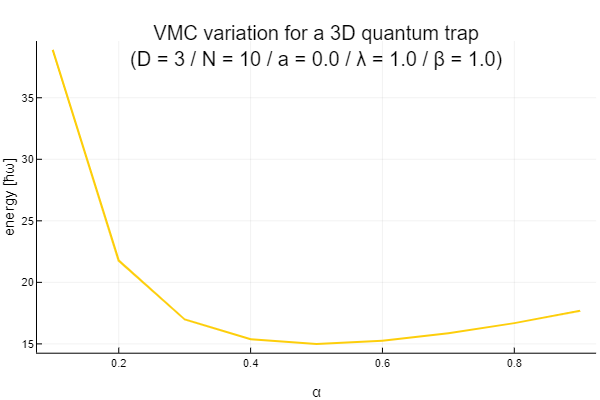
\includegraphics[width=0.9\columnwidth]{fig3D10_variation}
\captionof{figure}{\small Range variation for system \texttt{3D10} around the optimal value for $\alpha$, with the value for $\beta$ fixed at the optimal $1.0$. As expected, there is a clear minimum at ${\alpha = 0.5}$.}\label{var3D10}
\end{center}

More interesting are the range variation results for the interacting systems given in figures \ref{var3D10i} and \ref{var3D10ie}, which were varied around the optimal values for $\alpha$ and $\beta$ found with the gradient descent variation above. The resulting values for $\alpha$, $\beta$ and $E_\text{VMC}$ are given in table \ref{r3D10}.

\begin{center}
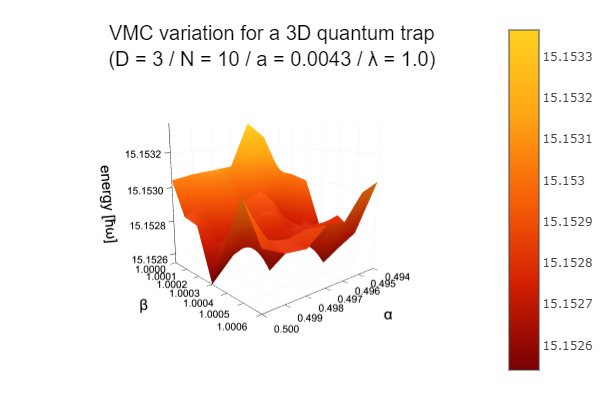
\includegraphics[width=0.9\columnwidth]{fig3D10i_variation}
\captionof{figure}{\small Range variation for the spherical interacting system \texttt{3D10i} around the optimal values for $\alpha$ and $\beta$ found with gradient descent variation (table \ref{gd3D10}). The minimum is less clear in this case.}\label{var3D10i}
\end{center}

\begin{center}
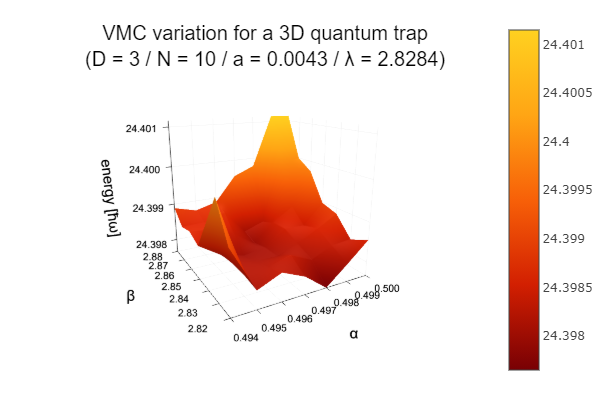
\includegraphics[width=0.9\columnwidth]{fig3D10ie_variation}
\captionof{figure}{\small Range variation for the elliptical interacting system \texttt{3D10ie} around the optimal values for $\alpha$ and $\beta$ found with gradient descent variation (table \ref{gd3D10}). The minimum is also here less clear.}\label{var3D10ie}
\end{center}

\begin{center}\small
\captionof{table}{\small Results of range variation for the 3-dimensional systems with 10 interacting bosons, based on the gradient descent results from table \ref{gd3D10}.}
\label{r3D10}
\begin{tabular}{cccr}
	\hline\hline
	System & Optimal $\alpha$ & Optimal $\beta$ & VMC energy \\
	\hline
    \texttt{3D10i} & $0.4970$ & $1.0006$ & $15.1525 \pm 0.0001$\\
    \texttt{3D10ie} & $0.4940$ & $2.8600$ & $24.3976 \pm 0.0007$\\
    \hline\hline
\end{tabular}
\end{center}

The found VMC energies are almost the same as the ones found with gradient descent, but this is due to the energy being approximately the same in the whole variational areas on the plots as much as due to anything else; while the range variation for \texttt{3D10ie} finds approximately the same minimum to 3-digit precision, the range variation for \texttt{3D10i} actually finds a \textit{new} minimum when compared to the results from gradient descent variation in table \ref{gd3D10}. Furthermore both plots reveal a chaotic energy surface across $\alpha$ and $\beta$, indicating that gradient descent could easily get caught in local minima for these systems. Hence, the apparent raising of $\beta$ discussed above might just be due to the numerical imprecision which is clearly in play here. The effect of bosonic interaction on the optimal values of $\alpha$ and $\beta$ will be examined further in section \ref{3Die}, in which elliptical traps with $10$, $50$ and $100$ interacting bosons are simulated.

As another test of expected results, the convergence of sampling methods for the interacting systems are plotted and compared in figures \ref{samp3D10i} and \ref{samp3D10ie}. In both plots it is clear that quantum drift sampling converges faster than random step sampling. Already at ${M = 10^4}$ Monte Carlo cycles, the QD-sampled VMC energy has converged pretty well. Looking also at the statistical error ribbons, the (block-resampled) error becomes smaller in the case of QD sampling when compared to RS sampling for $M > 10^3$. It hence seems that the quantum drift method indeed samples the important parts of configuration space earlier on, as discussed in section \ref{quantumdrift}.

\begin{center}
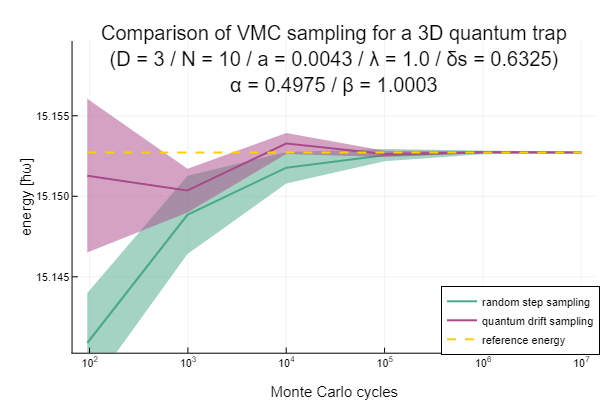
\includegraphics[width=0.9\columnwidth]{fig3D10i_sampling}
\captionof{figure}{\small Comparison of sampling methods for the spherical interacting system (\texttt{3D10i}) at the optimal values of $\alpha$ and $\beta$ found with gradient descent variation (table \ref{gd3D10}).}\label{samp3D10i}
\end{center}

\begin{center}
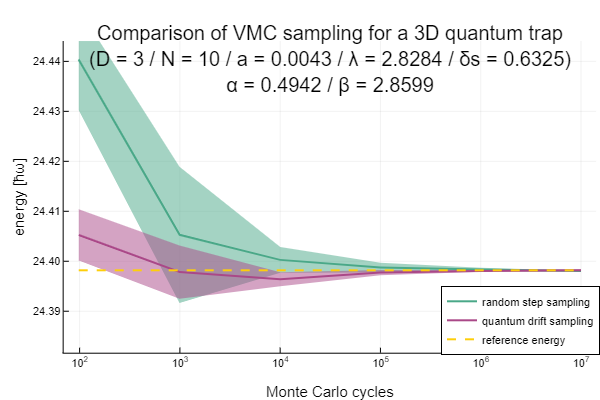
\includegraphics[width=0.9\columnwidth]{fig3D10ie_sampling}
\captionof{figure}{\small Comparison of sampling methods for the elliptical interacting system (\texttt{3D10ie}) around the optimal values for $\alpha$ and $\beta$ found with gradient descent variation (table \ref{gd3D10}).}\label{samp3D10ie}
\end{center}

Convergence of sampling methods for the non-interacting system \texttt{3D10} is plotted in figure \ref{samp3D10}. As expected after the discussion in section \ref{benchmarking}, both methods show definite convergence with no error, because the local energy is simply constant in this case. The plot for \texttt{3D10e} turned out similarly.\footnote{Actually, the plot for \texttt{3D10e} turned out \underline{almost} similarly, except for some strange numerical behaviour for some values of $M$, as can be seen in the folder \texttt{results} on GitHub. This is thought to be due to catastrophic cancellation or something of the kind.} 

\begin{center}
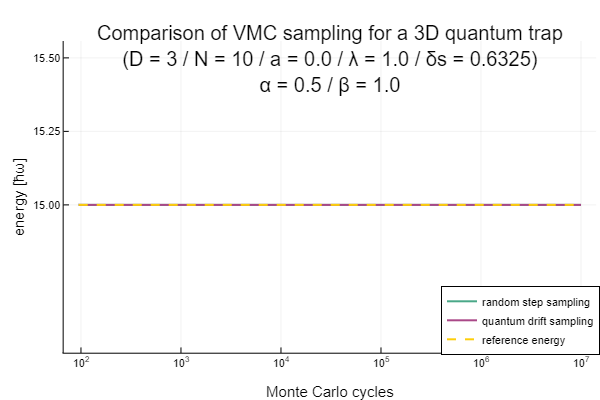
\includegraphics[width=0.9\columnwidth]{fig3D10_sampling}
\captionof{figure}{\small Comparison of sampling methods for the spherical non-interacting system (\texttt{3D10}) around the optimal values for $\alpha$ and $\beta$. Both methods converge from start.}\label{samp3D10}
\end{center}

As a conclusion to this section, block resampling of statistical error for system \texttt{3D10ie} is plotted in figure \ref{block3D10ie}. The resampled error grows with the number of blockings until reaching a maximum (in this case at 8), just as described in section \ref{Bresampling}.

\begin{center}
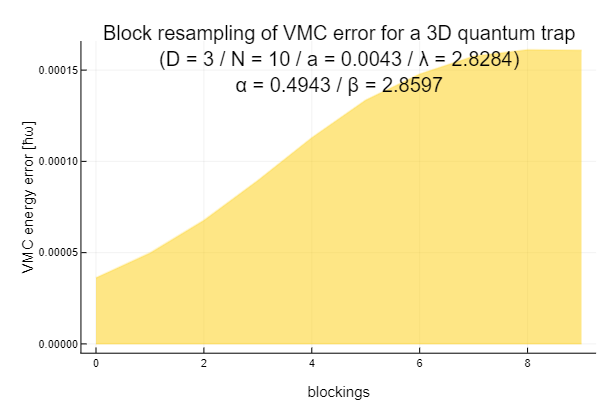
\includegraphics[width=0.9\columnwidth]{fig3D10ie_resampling}
\captionof{figure}{\small Block resampling of the statistical error for the elliptical interacting system (\texttt{3D10ie}).}\label{block3D10ie}
\end{center}

Having obtained output from the script which is mostly as expected, the main results of this report are presented in the next section.



\subsection{3-dimensional elliptical traps with 10, 50 and 100 interacting bosons}\label{3Die}
The gradient descent results for 3D traps with 10 bosons in table \ref{gd3D10} seemed to indicate that the optimal value for the elliptic variational parameter $\beta$ is raised when particle interaction is introduced to the system. The lowering of the optimal value for $\alpha$ is reported \cite{SWL}, but since they did not vary $\beta$, instead keeping it constant at ${\beta = \lambda = \sqrt{8} \approx 2.8284}$, they cannot strengthen the claim. Furthermore, the variational plots of figures \ref{var3D10i} and \ref{var3D10ie} display a chaotic energy surface for interacting systems which indicates the possibility of being trapped in a local minimum which could in the worst scenario be a result of statistical or numerical imprecision, rather than being a true minimum at all.

To examine the impact of particle interaction on $\beta$, elliptical traps with 10, 50 and 100 (hereafter referred to as \texttt{3D10ie}, \texttt{3D50ie} and \texttt{3D100ie}) interacting bosons are considered in deeper detail. The results of Schøyen and Winther-Larsen for these systems are presented in table \ref{SWLresults}.

\begin{center}\small
\captionof{table}{\small Results of Schøyen and Winther-Larsen\cite{SWL} for elliptical interacting systems, varying only the variational parameter $\alpha$.}
\label{SWLresults}
\begin{tabular}{cr}
	\hline\hline
	System & VMC energy \\
	\hline
    \texttt{3D10ie} & $24.3986 \pm 0.0003$\\
    \texttt{3D50ie} & $127.2852 \pm 0.0077$\\
    \texttt{3D100ie} & $266.2904 \pm 0.0297$\\
    \hline\hline
\end{tabular}
\end{center}

Starting at the optimal variational point of \cite{SWL}, which was found to be ${\alpha = 0.49744}$ and ${\beta = \lambda} = {\sqrt{8} \approx 2.8284}$, the three systems were gradient descended with the Julia script, varying both $\alpha$ and $\beta$ to search for an even lower VMC energy. All systems were gradient descended using the initial values ${\delta s = 0.0001}$ and $\delta g = 0.1$) given in section \ref{tuning}. As expected, the larger systems \texttt{3D50ie} and \texttt{3D100ie} were found to be more unstable with respect to gradient descent; while the smallest system was varied 4 successive times with increasing precision in $\delta v$ and $\delta g$, the larger systems were only varied 3 and 2 successive times, respectively, as gradient descent variation started to diverge. The full Julia output from the search is included in appendix \ref{gdOutput}, but the results are concisely summed up in table \ref{BFresults}. Interestingly, the raising of $\beta$ is demonstrated also in these results, and furthermore the raising increases with the number of bosons $N$. In fact, the relative raising of $\beta$ seems to be approximately \underline{equal} to the relative lowering of $\alpha$ when compared to the non-interacting optimal values ${\alpha = 0.5}$ and ${\beta = 2.8284}$, with respective relative changes $1\%$, $5\%$ and $9\%$ for 10, 50 and 100 bosons.

\begin{center}\small
\captionof{table}{\small Results of subsequent gradient descent for elliptical interacting systems, varying both variational parameters $\alpha$ and $\beta$. Convergence plots and full Julia output of the search is included in appendix \ref{output}.}
\label{BFresults}
\begin{tabular}{cccr}
	\hline\hline
	System & Optimal $\alpha$ & Optimal $\beta$ & VMC energy \\
	\hline
    \texttt{3D10ie} & $0.4943$ & $2.8597$ & $24.3979 \pm 0.0000$\\
    \texttt{3D50ie} & $0.4743$ & $2.9813$ & $127.2168 \pm 0.0004$\\
    \texttt{3D100ie} & $0.4581$ & $3.0957$ & $265.9246 \pm 0.0023$\\
    \hline\hline
\end{tabular}
\end{center}

The results of table \ref{BFresults} were controlled by running a final 100 million Monte Carlo cycles at the found optimal point, as shown in the output of appendix \label{output}. Convergence plots for all three values are given in section \ref{convOutput}, in which it becomes clear that the VMC energy converges already at 100 thousand Monte Carlo cycles for all three systems. This strengthens the validity of the results, as the last gradient descent was run with 100 thousand Monte Carlo cycles at each variational point. It also indicates that it is sufficient really to run only $M = 10^6$ Monte Carlo cycles in future simulations of these systems, which would of course greatly reduce the computation time.

As one last verification of the Julia script developed here, simulations for all three systems were also run at the optimal point ${\alpha = 0.49744}$ and ${\beta = \lambda = \sqrt{8}}$ found by Schøyen and Winther-Larsen, with the same number of Monte Carlo cycles, ${M = 2^21}$ and a sampling step size ${\delta s = \sqrt{0.1}}$ corresponding to their $\delta t = 0.1$. These parametric values are shown in table \ref{BFSWLresults} to reproduce their energy estimates to 1-digit precision, statistical errors also matching in magnitude.

\begin{center}\small
\captionof{table}{\small Reproduction of the results of Schøyen and Winther-Larsen\cite{SWL} for elliptical interacting systems, using the same parametric values as them.}
\label{BFSWLresults}
\begin{tabular}{cr}
	\hline\hline
	System & VMC energy \\
	\hline
    \texttt{3D10ie} & $24.3986 \pm 0.0003$\\
    \texttt{3D50ie} & $127.2818 \pm 0.0063$\\
    \texttt{3D100ie} & $266.3434 \pm 0.0328$\\
    \hline\hline
\end{tabular}
\end{center}

Having demonstrated overall consistent results with \cite{SWL}, one should of course also benchmark against other work, but there are not too many other viable results from the exact system of this report to be found. The seminal paper by DuBois and Glyde\cite{DBG} considers a greater range of systems, and does not explicitly present results for the three systems considered in this section. However, rescaling their figure 2 as done below, one clearly sees that the results found in this report, as well as the report of Schøyen and Winther-Larsen\cite{SWL}, both fall within the discernible range of their calculations.

\begin{center}
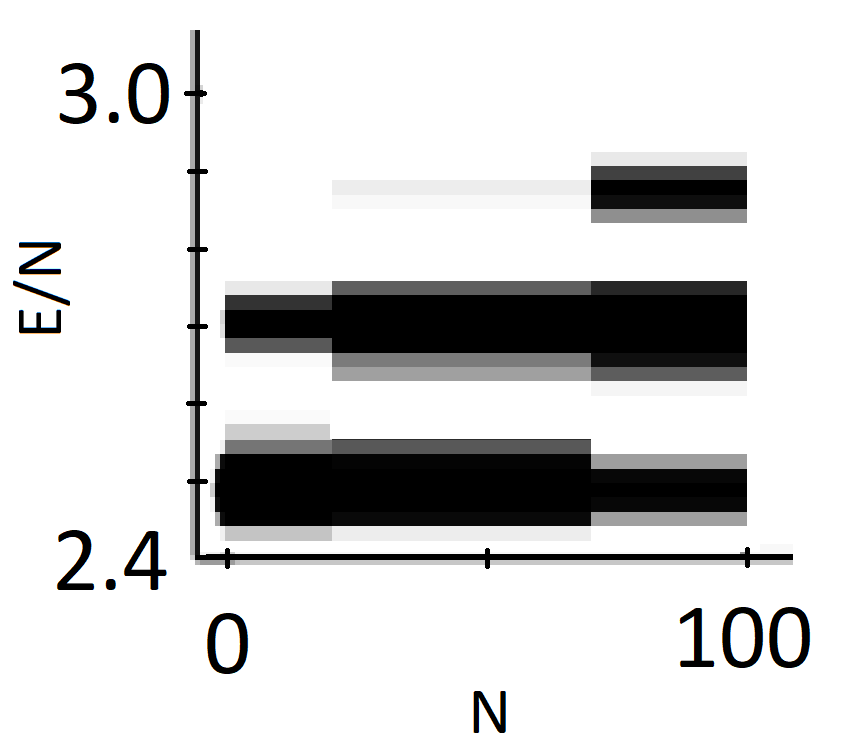
\includegraphics[width=0.9\columnwidth]{DBG_results}
\captionof{figure}{\small A rescaled presentation of the results of DuBois and Glyde\cite{DBG}. Their results discernably matches the results of this report as well as \cite{SWL}.}\label{DBGresults}
\end{center}

Note that the energy in figure \ref{DBGresults} is given per particle, so it should be multiplied respectively by 10, 50 and 100. In \cite{DBG} they used a Variational Monte Carlo approach similar to the one presented here, and it is reassuring to see that they obtain results of a similar scale to the results in tables \ref{SWLresults} and \ref{BFresults}.



\section{Conclusion}
In this report, the theoretical and computational development of a Variational Monte Carlo script written in the Julia language was presented, and it was run to both reproduce well-known results and produce novel results regarding the elliptic variational parameter $\beta$. For elliptical traps with 10, 50 and 100 interacting bosons, varying both $\alpha$ and $\beta$ resulted in slightly lower energy estimates than only varying $\alpha$ as done by Schøyen and Winther-Larsen. This lowering encourages further analysis of the optimal $\beta$ which is demonstrated here to be raised by introducing particle interaction to the system. However as the change in optimal $\beta$ is relatively small for the numbers of bosons considered here, the results of this report also validates the usual approximation ${\beta = \lambda}$ at least for systems with fewer than 100 particles.

Computational optimisation was done to the written Julia script with respect to storage, memory-handling and parallellisation, resulting in a total speed-up of more than 14. As the script was developed as a first-time experience with the Julia language, there is sure to be many more optimalisations which can further increase the speed of simulations. That said however, Julia performance better than C++ has seldom been reported, and only in special cases.

Despite the Julia script of this project being written with a specific bosonic harmonic trap system in mind, one could fairly easily extend it to perform Variational Monte Carlo on a broader range of quantum systems. To this end, numerical differentiation could be implemented to calculate the local energy for an arbitrary system, although as demonstrated in \cite{SWL} such calculations are prone to be very slow compared to analytical calculations such as the one derived in this report. The script could also be extended to sample and estimate other system obsevables of interest.

In \cite{NMPGHJP}, the very system considered in this report was treated, analytically and numerically, using Gross-Pitaevskii minimisation as well as Variational Monte Carlo, to obtain results for the ground state and vortex states of an elliptical trap with ${N = 500}$ interacting bosons with a large characteristic radius of ${a = 0.15155}$. Were the Julia script of this project to be further optimalised or run on a supercomputer, it could produce results for their trap system which could both verify their ground state estimates, but also lower the estimates further by raising $\beta$ as demonstrated.

While the script is ready for new adventures, the main goal of this project was to get acquainted with the Variational Monte Carlo method, computational optimalisation as well as the Julia language. In that regard it was a success. Braced and inspired by the computational lessons learned here, I will probably use both VMC and Julia again in future research.

\end{multicols}
\bibliographystyle{unsrt}
\bibliography{FYS9411_project1}


\newpage
\appendix
\setcounter{equation}{0}
\renewcommand{\theequation}{\thesection\arabic{equation}}
\section*{APPENDIX}
\section{Calculations}
Some of the longer analytical calculations of the project are presented here.


\subsection{Local energy $\varepsilon$}\label{derLocalenergy}
Equation \eqref{localenergy} defines the local energy $\varepsilon$ through the Hamiltonian $H$ given in \eqref{Ham} and the trial wavefunction $\Psi$ given in \eqref{trialstate}. The potential terms $U$ og $V$ in the Hamiltonian give direct contributions to the local energy, but the kinetic term with its second derivative $\vec{\nabla}_i^2\Psi$ needs to be considered further. To this end, write
\begin{equation}
\Psi[\vec{R}] = G[\vec{R}]F[\vec{R}]
\end{equation}
with
\begin{align}
G[\vec{R}] &= \prod\limits_i^N g[\vec{r}_i] \label{G}\\
F[\vec{R}] &= \prod\limits_j^N\prod\limits_{k > j}^N f[\Delta{r}_{jk}] \label{F}
\end{align}
and note that
\begin{equation}
\vec{\nabla}_i^2\Psi = \vec{\nabla}_i\cdot\left(\vec{\nabla}_i G F + G \vec{\nabla}_i F\right) = \vec{\nabla}_i^2 G F + 2\vec{\nabla}_i G \cdot \vec{\nabla}_i F + G \vec{\nabla}_i^2 F. \label{Lap_Psi_1} 
\end{equation}
Hence the derivatives of both $G$ and $F$ must be calculated in order to get an analytical expression for the local energy $\varepsilon$. The derivatives of $G$ are 
\begin{align}
\vec{\nabla}_i G &= \vec{\nabla}_i g[\vec{r}_i] \prod\limits_{j \neq i}^N g[\vec{r_j}] \nonumber\\
\Longrightarrow\quad \vec{\nabla}_i^2 G &= \vec{\nabla}_i^2 g[\vec{r}_i] \prod\limits_{j \neq i}^N g[\vec{r_j}], \nonumber
\end{align}
and because the derivatives of $g$ are
\begin{align}
\vec{\nabla}_i g[\vec{r}_i] &= -2\alpha\Big(\vec{x}_i+\vec{y}_i+\beta\vec{z}_i\Big)g[\vec{r}_i] \\
\Longrightarrow \vec{\nabla}_i^2 g[\vec{r}_i] &= -2\alpha\left(\Big(D+(\beta-1)\delta_{D,3}\Big)g[\vec{r}_i]+\Big(\vec{x}_i+\vec{y}_i+\beta\vec{z}_i\Big)\cdot\vec{\nabla}_i g[\vec{r}_i]\right) \nonumber\\
&= 2\alpha\left(2\alpha\Big(\vec{x}_i+\vec{y}_i+\beta\vec{z}_i\Big)^2-\Big(D+(\beta-1)\delta_{D,3}\Big)\right)g[\vec{r}_i]
\end{align}
where $\delta$ is the Kronecker delta, these are quite simply given by
\begin{align}
&\vec{\nabla}_i G = -2\alpha\Big(\vec{x}_i+\vec{y}_i+\beta\vec{z}_i\Big)G, \label{grad_G}\\
&\vec{\nabla}_i^2G = 2\alpha\left(2\alpha\Big(\vec{x}_i+\vec{y}_i+\beta\vec{z}_i\Big)^2-\Big(D+(\beta-1)\delta_{D,3}\Big)\right)G. \label{Lap_G}
\end{align}
To find the derivatives of $F$, rewrite the product in \eqref{F} to the exponential form 
\begin{equation}
F[\vec{R}] = \epsilon^{\sum\limits_{j}^N\sum\limits_{k > j}^N \ln f[\Delta{r}_{jk}]}
\end{equation}
and note that
\begin{align}
\vec{\nabla}_i F &= \sum\limits_{j \neq i}^N \left(\frac{\vec{\nabla}_i f[\Delta{r}_{ij}]}{f[\Delta{r}_{ij}]}\right) F \nonumber\\
\Longrightarrow \vec{\nabla}_i^2 F &= \sum\limits_{j \neq i}^N \left(\vec{\nabla}_i\cdot\left[\frac{\vec{\nabla}_i f[\Delta{r}_{ij}]}{f[\Delta{r}_{ij}]}\right]\right) F + \sum\limits_{j \neq i}^N \left(\frac{\vec{\nabla}_i f[\Delta{r}_{ij}]}{f[\Delta{r}_{ij}]}\right)\cdot \vec{\nabla}_i F \nonumber\\
&= \sum\limits_{j \neq i}^N \left(\frac{\vec{\nabla}_i^2 f[\Delta{r}_{ij}]}{f[\Delta{r}_{ij}]} - \frac{\left(\vec{\nabla}_i f[\Delta{r}_{ij}]\right)^2}{f^2[\Delta{r}_{ij}]}\right) F + \sum\limits_{j \neq i}^N \sum\limits_{k \neq i}^N \left(\frac{\vec{\nabla}_i f[\Delta{r}_{ij}] \cdot\vec{\nabla}_i f[\Delta{r}_{ik}]}{f[\Delta{r}_{ij}]f[\Delta{r}_{ik}]}\right) F \nonumber\\
&= \sum\limits_{j \neq i}^N \left(\frac{\vec{\nabla}_i^2 f[\Delta{r}_{ij}]}{f[\Delta{r}_{ij}]} + \sum\limits_{{k \neq i}\atop{k \neq j}}^N \frac{\vec{\nabla}_i f[\Delta{r}_{ij}] \cdot\vec{\nabla}_i f[\Delta{r}_{ik}]}{f[\Delta{r}_{ij}]f[\Delta{r}_{ik}]}\right) F. \nonumber
\end{align}
The derivatives of $f$ are
\begin{align}
\vec{\nabla}_i f[\Delta{r}_{ij}] &= \frac{a\Delta\vec{r}_{ij}}{\Delta{r}_{ij}^3} \\
\Longrightarrow \vec{\nabla}_i^2 f[\Delta{r}_{ij}] &= \frac{aD}{\Delta{r}_{ij}^3}-\frac{3a\Delta\vec{r}_{ij}^2}{\Delta{r}_{ij}^5} \nonumber\\
&= \frac{a(D-3)}{\Delta{r}_{ij}^3}
\end{align}
as long as all $\Delta{r}_{ij} > a$. Now since, by the definition \eqref{f}, 
\begin{equation}
\Delta{r}_{ij} f[\Delta{r}_{ij}] = \Delta{r}_{ij}-a \nonumber
\end{equation}
it follows that
\begin{align}
\vec{\nabla}_i F &= \sum\limits_{j \neq i}^N \left(\frac{a\Delta\vec{r}_{ij}}{\Delta{r}_{ij}^2(\Delta{r}_{ij}-a)}\right) F, \label{grad_F}\\
\vec{\nabla}_i^2 F &= \sum\limits_{j \neq i}^N \left(\frac{a(D-3)}{\Delta{r}_{ij}^2(\Delta{r}_{ij}-a)} + \sum\limits_{{k \neq i}\atop{k \neq j}}^N \frac{a^2 \Delta\vec{r}_{ij} \cdot \Delta\vec{r}_{ik}}{\Delta{r}_{ij}^2(\Delta{r}_{ij}-a) \Delta{r}_{ik}^2(\Delta{r}_{ik}-a)}\right) F. \label{Lap_F}
\end{align}

Then in total equation \eqref{Lap_Psi_1} takes the form
\begin{align}
\vec{\nabla}_i^2\Psi &= 2\alpha\left(2\alpha\Big(\vec{x}_i+\vec{y}_i+\beta\vec{z}_i\Big)^2-\Big(D+(\beta-1)\delta_{D,3}\Big)\right) \Psi \nonumber\\
&- 4\alpha\Big(\vec{x}_i+\vec{y}_i+\beta\vec{z}_i\Big) \cdot \sum\limits_{j \neq i}^N \left(\frac{a\Delta\vec{r}_{ij}}{\Delta{r}_{ij}^2(\Delta{r}_{ij}-a)}\right) \Psi \nonumber\\
&+ \sum\limits_{j \neq i}^N \left(\frac{a(D-3)}{\Delta{r}_{ij}^2(\Delta{r}_{ij}-a)} + \sum\limits_{{k \neq i}\atop{k \neq j}}^N \frac{a^2 \Delta\vec{r}_{ij} \cdot \Delta\vec{r}_{ik}}{\Delta{r}_{ij}^2(\Delta{r}_{ij}-a) \Delta{r}_{ik}^2(\Delta{r}_{ik}-a)}\right) \Psi \nonumber\\
\Longrightarrow \frac{\vec{\nabla}_i^2\Psi}{\Psi} &= 2\alpha\left(2\alpha\Big(\vec{x}_i+\vec{y}_i+\beta\vec{z}_i\Big)^2-\Big(D+(\beta-1)\delta_{D,3}\Big)\right) \nonumber\\
&+ \sum\limits_{j \neq i}^N \frac{a(D-3) - 4\alpha\Big(\vec{x}_i+\vec{y}_i+\beta\vec{z}_i\Big) \cdot a\Delta\vec{r}_{ij}}{\Delta{r}_{ij}^2(\Delta{r}_{ij}-a)} \nonumber\\
&+ \sum\limits_{j \neq i}^N \sum\limits_{{k \neq i}\atop{k \neq j}}^N \frac{a^2 \Delta\vec{r}_{ij} \cdot \Delta\vec{r}_{ik}}{\Delta{r}_{ij}^2(\Delta{r}_{ij}-a) \Delta{r}_{ik}^2(\Delta{r}_{ik}-a)}
\end{align}
and by introducing the quantities
\begin{align}
\vec{q}[\vec{r}_i] &= -4\alpha\Big(\vec{x}_i+\vec{y}_i+\beta\vec{z}_i\Big), \label{q}\\
d[\Delta{r}_{ij}] &= \Delta{r}_{ij}^2(\Delta{r}_{ij}-a), \label{d}\\
\vec{s}[\Delta\vec{r}_{ij}] &= \frac{a\Delta\vec{r}_{ij}}{2d[\Delta{r}_{ij}]}, \label{s}
\end{align}
it follows that the total analytic expression for the local energy is
\begin{align}
\varepsilon[\vec{R}] &= \alpha N\Big(D+(\beta-1)\delta_{D,3}\Big) + \sum\limits_i^N \frac{1}{2}\left( U[\vec{r}_i] - \frac{1}{4}\vec{q}^2[\vec{r}_i] \right) \nonumber\\
&- \sum\limits_i^N \sum\limits_{j \neq i}^N \left( \frac{a(D-3)}{2d[\Delta{r}_{ij}]} + \vec{q}[\vec{r}_i] \cdot \vec{s}[\Delta\vec{r}_{ij}] \right) - 2\sum\limits_i^N \sum\limits_{j \neq i}^N \sum\limits_{{k \neq i}\atop{k \neq j}}^N \vec{s}[\Delta\vec{r}_{ij}] \cdot \vec{s}[\Delta\vec{r}_{ik}] \label{compLocalenergy}
\end{align}
as long as all $\Delta r_{ij} > a$. This last restriction is why the hard-sphere interaction energy $V$ is omitted altogether; for configurations in which $\Delta r_{ij} \leq a$ for some $i$ and $j$, the trial wavefunction $\Psi$ in \eqref{trialstate} is defined to be zero (because $f[\Delta r_{ij}]$ is zero), which in turn means that the Metropolis algorithm will never sample such configurations, and so the fact that the local energy would be infinite for such configurations (because $V$ is infinite) is not a problem.


\subsection{Quantum drift $\vec{Q}$}\label{derQuantumdrift}
Equation \eqref{quantumdrift} defines the quantum drift of the system. From the formulas \eqref{grad_G} and \eqref{grad_F} of section \ref{derLocalenergy} it follows that
\begin{align}
\vec{\nabla}_i\Psi &= \vec{\nabla}_i G F + G \vec{\nabla}_i F \nonumber\\
&= -2\alpha\Big(\vec{x}_i+\vec{y}_i+\beta\vec{z}_i\Big)\Psi + \sum\limits_{j \neq i}^N \left(\frac{a\Delta\vec{r}_{ij}}{\Delta{r}_{ij}^2(\Delta{r}_{ij}-a)}\right) \Psi \nonumber\\
\Longrightarrow \frac{\vec{\nabla}_i\Psi}{\Psi} &= -2\alpha\Big(\vec{x}_i+\vec{y}_i+\beta\vec{z}_i\Big) + \sum\limits_{j \neq i}^N \left(\frac{a\Delta\vec{r}_{ij}}{\Delta{r}_{ij}^2(\Delta{r}_{ij}-a)}\right),
\end{align}
which means that the analytic expression for the quantum drift becomes
\begin{equation}
\vec{Q}_i[\vec{R}] = \vec{q}[\vec{r}_i] + 4\sum\limits_{j \neq i}^N \vec{s}[\Delta\vec{r}_{ij}]. \label{compQD}
\end{equation}
with the quantities introduced in \eqref{q}–\eqref{s}.


\subsection{Variational gradient $\frac{\partial\ev{\varepsilon}_\Pi}{\partial\alpha_i}$} \label{derVargrad}
The energy bound $\ev{\varepsilon}_\Pi$ introduced in section \ref{varmethod} is given by
\begin{equation}
\ev{\varepsilon}_\Pi = \frac{\idotsint \Psi^2[\vec{R}] \varepsilon[\vec{R}] \delta^{DN}R}{\idotsint \Psi^2[\vec{R}]\delta^{DN}R} \label{energybound}
\end{equation}
in the case of a real trial state $\Psi$ such as the one defined in \eqref{trialstate} and considered here. Denoting the variational parameters as $\alpha_i$ for $i \in \{1,2\}$ such that $\alpha_1 = \alpha$ and $\alpha_2 = \beta$, it is relevant for gradient descent variation as discussed in section \ref{gradientdescent} to calculate the variational gradient $\frac{\partial \ev{\varepsilon}_\Pi}{\partial \alpha_i}$. As both $\Psi$ and $\varepsilon$ depends on $\alpha_i$, the gradient is
\begin{align}
\frac{\partial\ev{\varepsilon}_\Pi}{\partial\alpha_i} &= \frac{\idotsint \left(2\Psi\frac{\partial\Psi}{\partial\alpha_i}\varepsilon+\Psi^2\frac{\partial\varepsilon}{\partial\alpha_i}\right)\delta^{DN}R}{\idotsint \Psi^2 \delta^{DN}R} - \frac{\idotsint \Psi^2\varepsilon \delta^{DN}R}{\idotsint \Psi^2 \delta^{DN}R}\frac{\idotsint 2\Psi\frac{\partial\Psi}{\partial\alpha_i}\delta^{DN}R}{\idotsint \Psi^2 \delta^{DN}R} \nonumber\\
&= \frac{\idotsint \left(2\Psi^2\frac{\partial\Psi}{\Psi\partial\alpha_i}\varepsilon+\Psi^2\frac{\partial\varepsilon}{\partial\alpha_i}\right)\delta^{DN}R}{\idotsint \Psi^2 \delta^{DN}R} - \frac{\idotsint \Psi^2\varepsilon \delta^{DN}R}{\idotsint \Psi^2 \delta^{DN}R}\frac{\idotsint 2\Psi^2\frac{\partial\Psi}{\Psi\partial\alpha_i}\delta^{DN}R}{\idotsint \Psi^2 \delta^{DN}R} \nonumber\\
&= \idotsint \left(2\Pi\frac{\partial\ln\Psi}{\partial\alpha_i}\varepsilon+\Pi\frac{\partial\varepsilon}{\partial\alpha_i}\right)\delta^{DN}R - \idotsint \Pi\varepsilon \delta^{DN}R \idotsint 2\Pi\frac{\partial\ln\Psi}{\partial\alpha_i} \delta^{DN}R \nonumber\\
&= 2\ev{\frac{\partial\ln\Psi}{\partial\alpha_i}\varepsilon}_\Pi-2\ev{\frac{\partial\ln\Psi}{\partial\alpha_i}}_\Pi\ev{\varepsilon}_\Pi+\ev{\frac{\partial\varepsilon}{\partial\alpha_i}}_\Pi. 
\end{align}
However the expected value of the variational derivative $\frac{\partial\varepsilon}{\partial\alpha_i}$ turns out to be zero,
\begin{align}
\ev{\frac{\partial\varepsilon}{\partial\alpha_i}}_\Pi &= \frac{\idotsint\Psi^2\frac{\partial}{\partial\alpha_i}\left[\frac{H[\Psi]}{\Psi}\right]\delta^{DN}R}{\idotsint \Psi^2 \delta^{DN}R} \nonumber\\
&= \frac{\idotsint\left(H\left[\frac{\partial\Psi}{\partial\alpha_i}\right]\Psi-H[\Psi]\frac{\partial\Psi}{\partial\alpha_i}\right)\delta^{DN}R}{\idotsint \Psi^2 \delta^{DN}R} = \frac{\bra{\Psi}\mathbf{H}\ket{\frac{\partial\Psi}{\partial\alpha_i}}-\bra{\Psi}\mathbf{H}^\dagger\ket{\frac{\partial\Psi}{\partial\alpha_i}}}{\braket{\Psi}{\Psi}} = 0,
\end{align}
so the variational gradient reduces to
\begin{equation}
\frac{\partial\ev{\varepsilon}_\Pi}{\partial\alpha_i} = 2\ev{\frac{\partial\ln\Psi}{\partial\alpha_i}\varepsilon}_\Pi-2\ev{\frac{\partial\ln\Psi}{\partial\alpha_i}}_\Pi\ev{\varepsilon}_\Pi.
\end{equation}
The expected values in this expression can be estimated by sampling the quantities
\begin{align}
\frac{\partial\ln\Psi}{\partial\alpha}[\vec{R}] &= -\sum\limits_i^N \left(x_i^2 + y_i^2 + \beta z_i^2\right), \label{compAlphaGrad}\\
\frac{\partial\ln\Psi}{\partial\beta}[\vec{R}] &= -\sum\limits_i^N \alpha z_i^2, \label{compBetaGrad}
\end{align}
as well as their product with the local energy $\varepsilon$, at each Monte Carlo cycle and then calculate their average when the averages of $\ev{\varepsilon}$ and $\ev{\varepsilon^2}$ are calculated.


\newpage
\section{Output}\label{output}
Some of the output from the Julia script developed for the project is included here for reference. The rest can be found in the folder \texttt{results} on GitHub\footnote{\texttt{https://github.com/flarrek/FYS9411-Project-1}}.

\subsection{Convergence of results for the systems \texttt{3D10ie}, \texttt{3D50ie} and \texttt{3D100ie}}\label{convOutput}

\begin{figure}[h!]
\centering
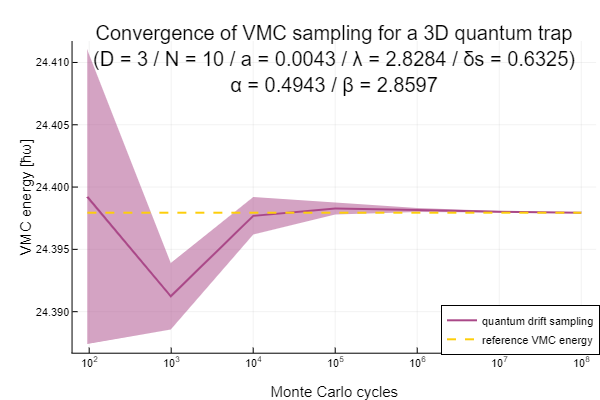
\includegraphics[height=0.22\textheight]{fig3D10ie_BF_convergence}
\captionof{figure}{\small Convergence of VMC energy for the elliptical trap with 10 interacting bosons (\texttt{3D10ie}).}
\end{figure}

\begin{figure}[h!]
\centering
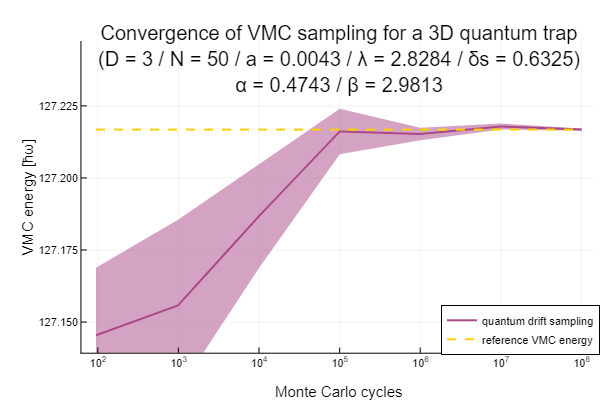
\includegraphics[height=0.22\textheight]{fig3D50ie_BF_convergence}
\captionof{figure}{\small Convergence of VMC energy for the elliptical trap with 50 interacting bosons (\texttt{3D50ie}).}
\end{figure}

\begin{figure}[h!]
\centering
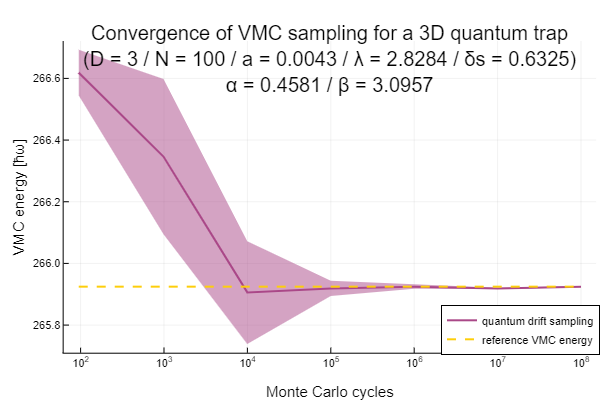
\includegraphics[height=0.22\textheight]{fig3D100ie_BF_convergence}
\captionof{figure}{\small Convergence of VMC energy for the elliptical trap with 100 interacting bosons (\texttt{3D100ie}).}
\end{figure}

\newpage
\subsection{Gradient descent variation of the systems \texttt{3D10ie}, \texttt{3D50ie} and \texttt{3D100ie}}\label{gdOutput}

\begin{figure}[h!]
\centering
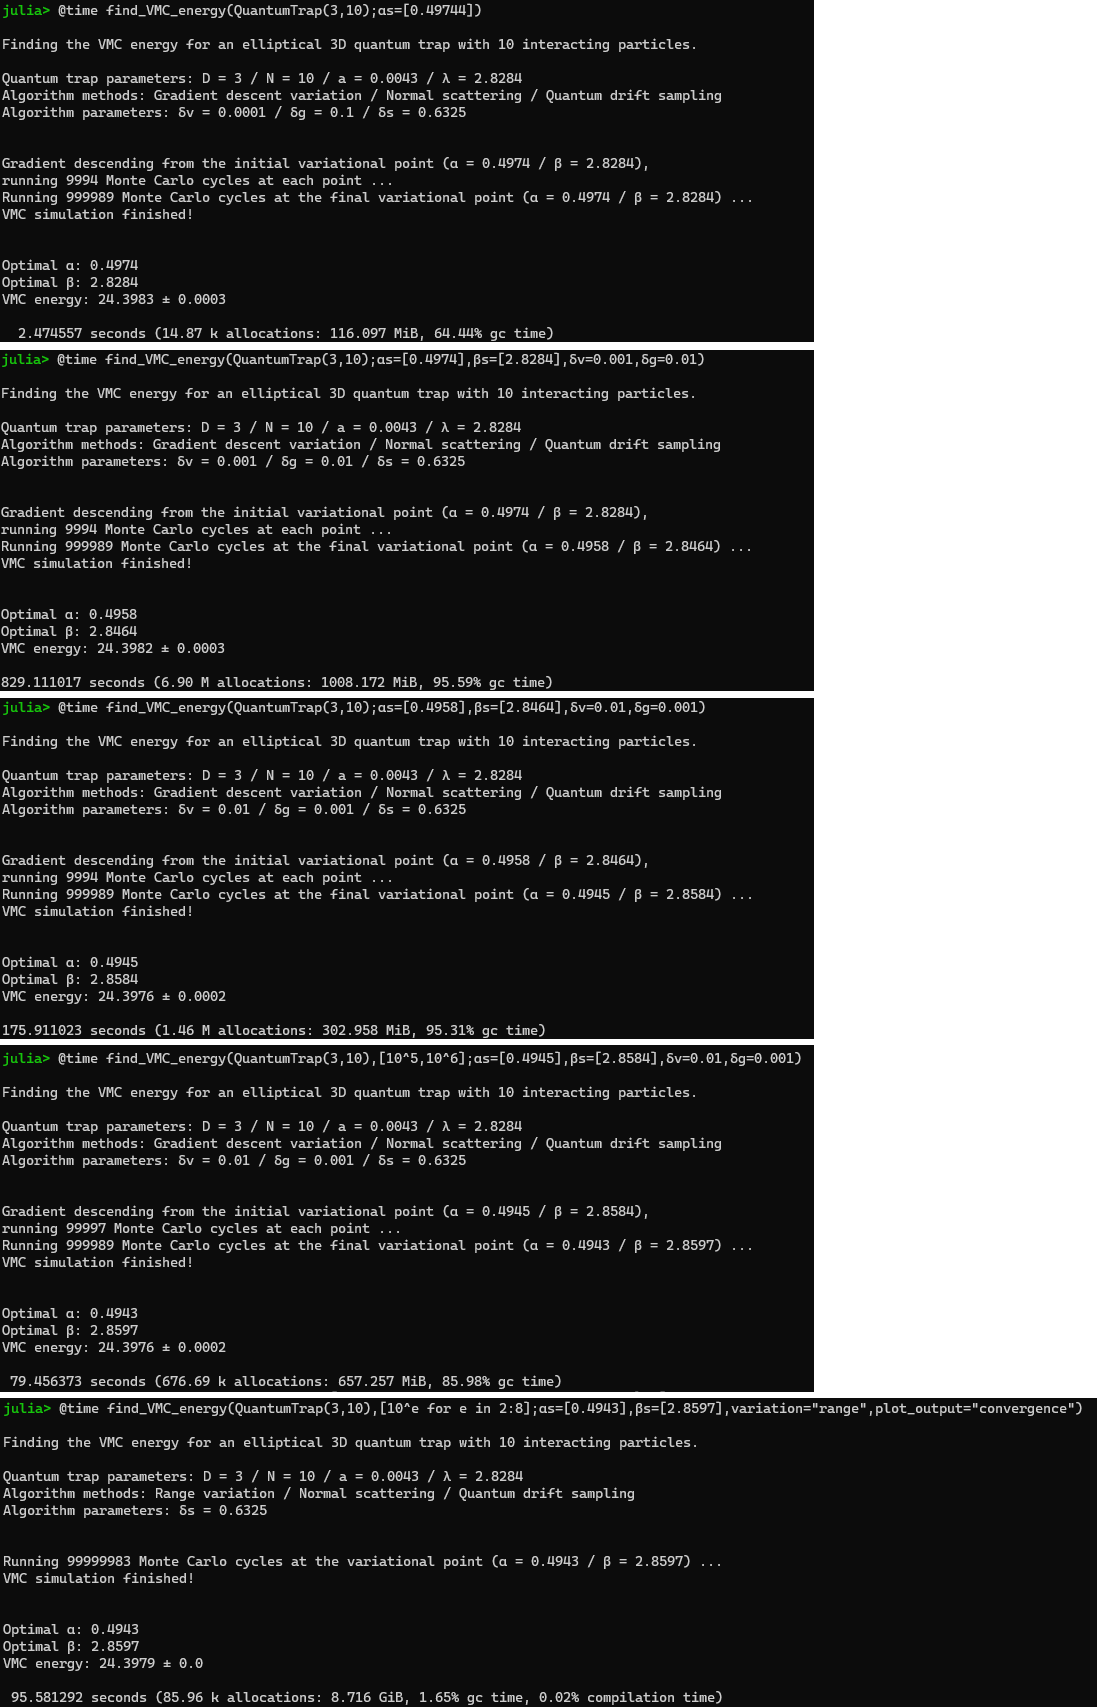
\includegraphics[width=0.8\textwidth]{fig3D10ie_search}
\captionof{figure}{\small Output from gradient descent variation and subsequent refinement of the elliptical trap with 10 interacting bosons (\texttt{3D10ie}).}
\end{figure}

\begin{figure}[h!]
\centering
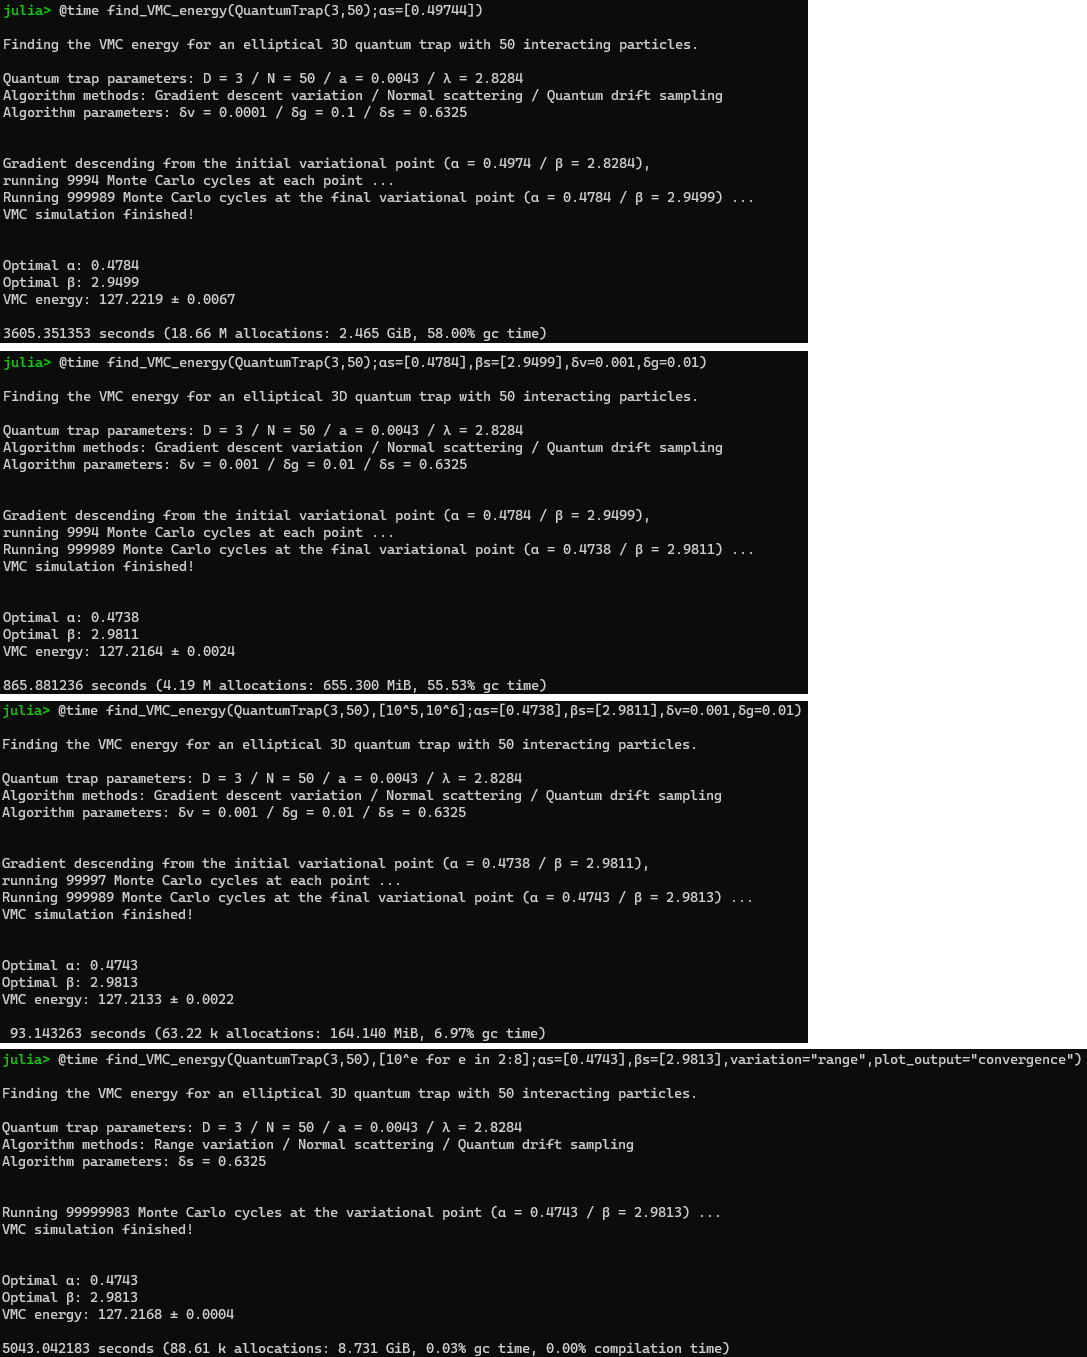
\includegraphics[width=0.8\textwidth]{fig3D50ie_search}
\captionof{figure}{\small Output from gradient descent variation and subsequent refinement of the elliptical trap with 50 interacting bosons (\texttt{3D50ie}).}
\end{figure}

\begin{figure}[h!]
\centering
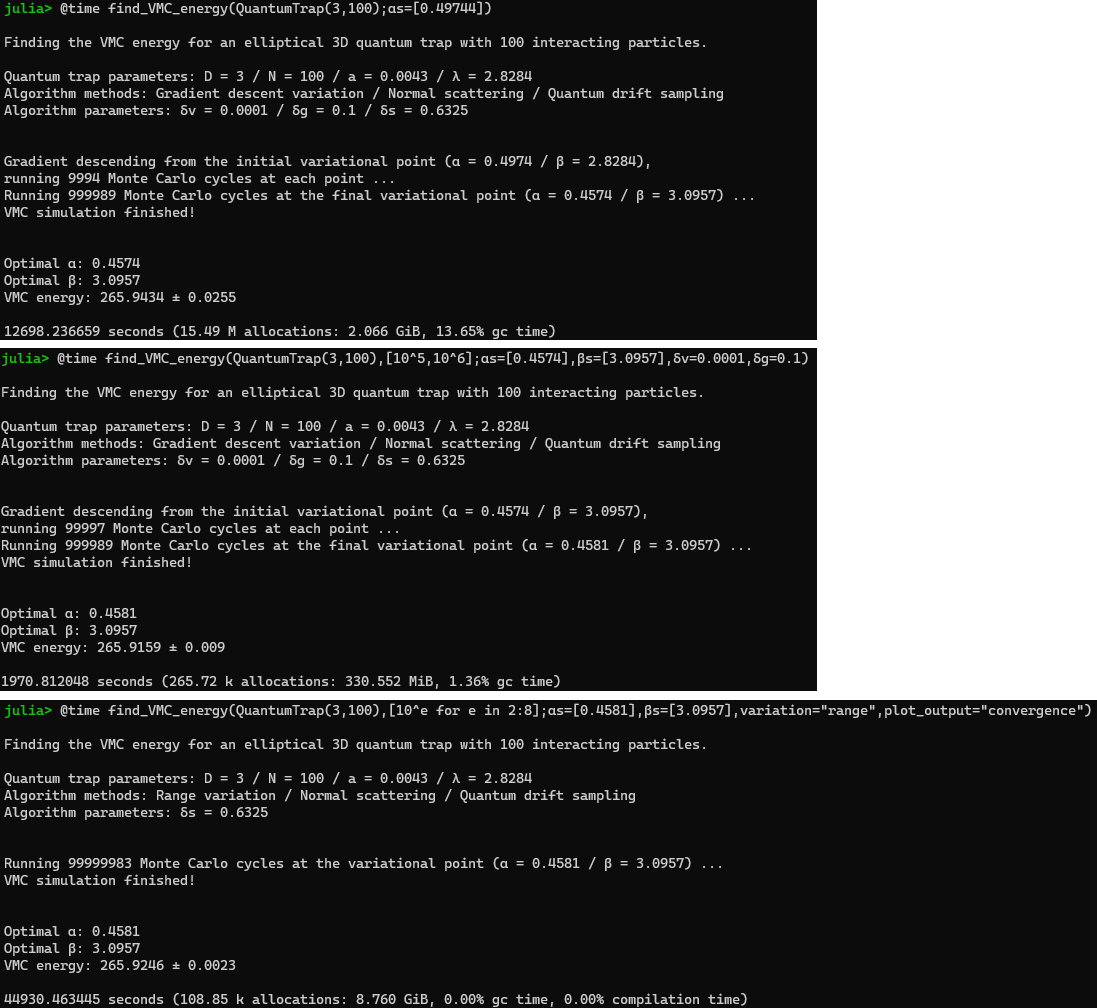
\includegraphics[width=0.8\textwidth]{fig3D100ie_search}
\captionof{figure}{\small Output from gradient descent variation and subsequent refinement of the elliptical trap with 100 interacting bosons (\texttt{3D100ie}).}
\end{figure}


\end{document}